\vspace*{1pc}


The Code for Anisotropies in the Microwave Background, or \texttt{CAMB}\footnote{\url{http://camb.info}} \citep{Lewis2000} is a
numerical Boltzmann code written in Fortran 90. It is a parallelized line-of-sight integration code which is widely used (and thus tested) to calculate not only
the lensed cosmic microwave background temperature and polarization spectra but also linear matter power spectra for different
species of particles (in our case baryons, dark matter and sometimes neutrinos). The Cosmic Linear Anisotropy Solving System, or \texttt{CLASS}\footnote{\url{http://class-code.net/}} \citep{CLASS} is a newer code  similar to \texttt{CAMB} with additional features such as the option of inputing a non-cold dark matter particle momentum distribution function, which was crucial for one of the projects I managed, involving resonantly-produced sterile neutrinos as a cool dark matter candidate particle (see Sec.~\ref{sec:rpsn_intro}).



%%%%%%%%%%%%%%%%%%%%%%%%%%%%%%%%%%%%%%%%%%%
\subsection{Power Spectrum of $\Lambda$CDM}
%%%%%%%%%%%%%%%%%%%%%%%%%%%%%%%%%%%%%%%%%%%

\subsubsection{Initial Conditions}
\label{sec:primordialps}

The 10 small perturbation variables ($\delta_{\mathrm{dm}, b, \nu}, v_{\mathrm{dm}, b, \nu}, \theta_{\gamma, \nu}, \phi, \psi$) obey the set of 10 first-order differential equations~\ref{eq:summary_euler}~\ref{eq:summary_poisson}. In principle, solving for the perturbations requires initial conditions for all 10 of them. However, in practice, when one assumes conformal times early enough so that any relevant $k$ mode verify $k \tau \ll 1$, a lot of simplifications can be taken advantage of to relate all of the required initial conditions to those on $\phi$ alone. Indeed, perturbations which have a wavelength $\lambda \sim k^{-1}$ at early times very large compared to the length scale at which causal physics applies (the horizon), all time derivative terms ($\propto \tau^{-1}$) are larger than gradient terms ($\propto k$) by a factor of order $\mathcal{O}(1/k\tau)$ which is large by assumption. Therefore the 8 Boltzmann equations in~\ref{eq:summary_euler} boil down to only the following 4\footnote{massless neutrinos obey the first involving its temperature monopole. The second involving their density only apply to the massive case} under this assumption:

\begin{equation}
\left\{ \begin{array}{ll}
\dot{\Theta}_{0, r} + \dot{\phi} = 0 & r \in \lbrace \gamma, \nu \rbrace \\
\\
\dot{\delta}_m - 3 \dot{\phi} = 0 & m \in \lbrace \mathrm{dm}, b, \nu \rbrace
\end{array}
\right.
\end{equation} \\

All velocity terms are smaller by a $\mathcal{O}(k \tau)$ factor, as are higher multipolar moments of the temperature distribution. For the baryon population, the tight coupling limit is valid, meaning the velocity term is exactly linked to the temperature dipole, set by the large value of $\dot{\tau}_{\mathrm{Compton}}$ (see Eq.~\ref{eq:tcl}): \\

\begin{equation}
v_b + 3 i \Theta_{1, \gamma} = 0
\end{equation} \\

Combining the Einstein equations (Eq.~\ref{eq:summary_poisson}) at very early times yield a second-order differential equation on the gravitational potential \\

\begin{equation}
\tau \ddot{\phi} + 4 \dot{\phi} = 0 
\end{equation} which admits 2 solutions if we assume $\phi \sim \tau^p$ is polynomial: $\phi \propto \tau^{-3} + \tau^0$. The first mode is decaying so even if it is excited at early times, it soon vanishes with respect to the constant mode. This mode yields $\dot{\phi} = 0 \Rightarrow \dot{\theta} = 0 \Rightarrow \theta = \mathrm{cst}, \delta = \mathrm{cst}, \delta_b = \mathrm{cst}$ and so in summary, if we equal both massless neutrino and photon temperature monopoles at early times: \\

\begin{equation}
\left\{
\begin{array}{l}
\Theta_{0, \nu} (k, \tau_{\mathrm{ic}}) = \Theta_{0, \gamma} (k, \tau_{\mathrm{ic}}) \doteq \Theta_{0} (k, \tau_{\mathrm{ic}}) \\
\\
\phi_0 (k, \tau_{\mathrm{ic}})  = 2 \Theta_{0} (k, \tau_{\mathrm{ic}}) \\
\\
\delta_m (k, \tau_{\mathrm{ic}}) - 3 \Theta_0 (k, \tau_{\mathrm{ic}}) = A
\end{array}
\right.
\end{equation} \\

So, solving for perturbations only requires the knowledge of 3 constants: $\Theta_0, \phi_0 ~\&~ A$, the last one of which depends on the nature of the primordial perturbations: \\

\begin{itemize}

\item[$\bullet$] adiabatic perturbations: $A = 0$ \\

\item[$\bullet$] isocurvature perturbations: $A \neq 0$ \\

\end{itemize}

 
Adiabatic perturbations feature a constant matter-to-radiation ratio everywhere since

\begin{equation*}
\frac{n_{\mathrm{dm}}}{n_{\gamma}} = \frac{n_{\mathrm{dm}}^0 (1+\delta)}{n^0_{\gamma} (1+3\Theta_0)} \simeq \frac{n^0_{\mathrm{dm}}}{n^0_{\gamma}} (1+\underbrace{\delta-3\Theta_0}_{0~ \text{if adiabatic}})
\end{equation*} and likewise for the baryon-to-entropy ratio $\eta_b = n_b / n_\gamma$. The standard model of cosmology assumes adiabatic scale invariant initial conditions. As such, all perturbations can be solved with the knowledge of a single function: the \textbf{primordial power spectrum} $\vert \phi(\vec{k}, \tau_{\mathrm{ic}} \ll \tau_{\mathrm{eq}}) \vert^2$ where $k \tau_{\mathrm{eq}} \simeq 1$. It is assumed to follow the expression for the Harison-Zel'dovich initial power spectrum (set by inflation) \\

\begin{empheq}[box=\mymath]{equation}
\label{def:Harrison}
k^3 ~ \left\vert \phi_{s,t}(\vec{k}, \tau_{\mathrm{ic}}) \right\vert^2 \simeq \mathcal{A}_{s,t} ~ k^{n_{s,t} - 1}
%\end{equation}
\end{empheq} \\
where $n=1$ for scale invariance and the $s$ and $t$ subscripts stand for the scalar and tensor modes of perturbations. As I've specified earlier in this chapter, I only consider scalar modes. I shall also mention that I am working under the gaussian assumption, meaning that $\phi$ is chosen such that its variance is its power spectrum $\vert \phi \vert^2$.\\

The assumption of decoupled modes at very early times enabled us to set the evolution of perturbations in density, velocity (and its divergence), temperature multipoles and gravitational potentials to solely the power spectrum of $\phi$, which is fully determined by an amplitude $\mathcal{A}_s$ and a spectral index $n_s$ for scalar modes, under the axiom that initial conditions are adiabatic and scale invariant. The CMB for instance can be fully determined by $\mathcal{A}_s$, $n_s$, the running of the scalar spectral index $d ns / d \ln k$, the ration of scalar to tensor power spectra $r$ and the optical depth to reionization $\tau_{\star}$. I should mention that although isocurvature pertubations are seldom used, these lead to 
\begin{equation}
\Theta_{1, r} = \frac{i v_m}{3} = - \frac{k \phi}{6 a H}
\end{equation} and so the power spectrum of $\phi$ determines each $k$ mode of all perturbations of interest as well.\\

In Sec.~\ref{sec:PS}, I introduced the formal definitions of power spectra for temperature and density fluctuations in radiation and density distributions. I've shown how they relate to the variance in their field and help quantify inhomogeneities and anisotropies. In the present Sec.~\ref{sec:CAMB}, I detail how the mass of neutrinos and dark matter particles impact the power spectrum through their free-streaming. 


\subsubsection{Pure Cold Dark Matter}


\begin{figure}
\begin{center}
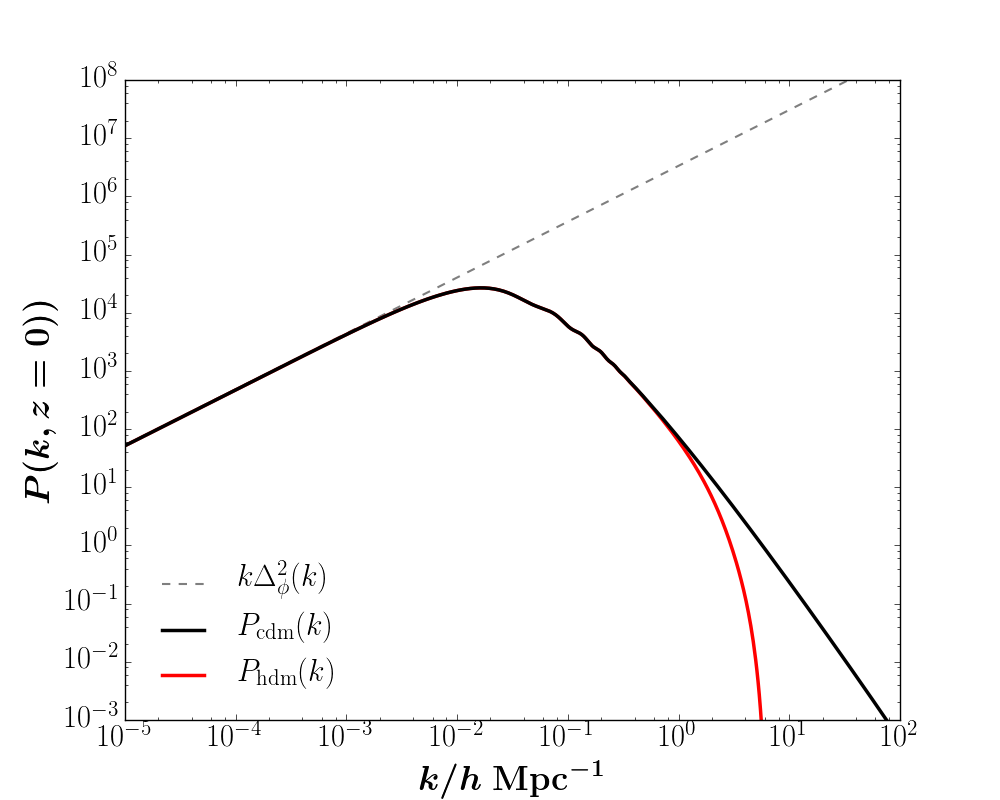
\includegraphics[width=0.8\columnwidth]{Pcdm_ic.png}
\caption{Power spectra of the matter distribution at $z=0$ in a standard $\Lambda$CDM model (thick solid black curve) and a pure $\Lambda$HDM model (thick solid red curve). The CDM transfer function $\mathcal{T}(k)$ defined in Eqs.~\ref{def:cdm_tf},\ref{eq:cdm_tf} is the ratio (square rooted) between the CDM power spectrum and that of the scalar modes of linear perturbations given by Eq.~\ref{def:Harrison} (grey dashed curve). The HDM transfer function $T(k)$ is the (square rooted) ratio between the HDM and CDM power spectra.}
\label{fig:initialpwrspc}
\end{center}
\end{figure}

The power spectrum of dark matter today at $\tau_0$ can be linked to the power spectrum of gravitational potential via the Poisson equation

\begin{align*}
P_{\mathrm{dm}} (\vec{k}, \tau_0) &\doteq \langle ~ \left\vert \tilde{\delta}_{\mathrm{dm}} (\vec{k}, \tau_0) \right\vert^2 ~ \rangle \\
&= \left( \frac{2}{3} \right)^2 \left( \frac{k}{H_0} \right)^{4} ~ \langle ~ \left\vert \tilde{\phi} (\vec{k}, \tau_0) \right\vert^2 ~ \rangle
\end{align*}

For $k$ modes that enter the horizon during the matter dominated era, \textit{i.e.} $k < k_{\mathrm{eq}} = 1 / \tau_{\mathrm{eq}}$, the current power spectrum of $\phi$ is the primordial Harrison Zel'dovich spectrum introduced in Eq.~\ref{def:Harrison}. Therefore the dark matter power spectrum today is proportional to\\
\begin{equation}
\label{eq:pkcdm_lowk}
P_{\mathrm{dm}} (k < k_{\mathrm{eq}}, \tau_0) \propto k \Delta^2_\phi
\end{equation} with $\delta^2_\phi \propto k^3 \langle \vert \phi \vert^2 \rangle$ which is scale invariant for $n_s = 1$. DM density fluctuations grow as $k$ at the largest scales (beyond equality), as displayed in the left part of Fig.~\ref{fig:initialpwrspc}. The black curve denoting the cold dark matter breaks away from the dotted curve, denoting the limit $k_{\mathrm{eq}} \rightarrow \infty$ for Eq.~\ref{eq:pkcdm_lowk}, at length scales smaller than the equality scale. Larger modes $k > k_{\mathrm{eq}}$ spend some amount of time, from $\tau = k^{-1}$ to $\tau_{\mathrm{eq}}$ inside the horizon during the radiation dominated era. During that time, $\phi \propto \tau^{-2}$ and so the relative suppression in its power spectrum is proportional to $(\tau / \tau_{\mathrm{eq}})^4 = (k_{\mathrm{eq}}/k)^4$. Hence the dark matter power spectrum asymptotically falls as $k^{-4}$ for large $k$ modes on Fig.~\ref{fig:initialpwrspc}. We can define the cold dark matter transfer function $\mathcal{T}(k)$ as
\begin{equation}
\label{def:cdm_tf}
P_{\mathrm{dm}} (k) ~ = ~ \mathcal{T}^2 (k) ~ P_{k_{\mathrm{eq}} \rightarrow \infty} (k)
\end{equation} where the right-most term (dashed line in Fig.~\ref{fig:initialpwrspc}) given by Eq.~\ref{eq:pkcdm_lowk} assumes no radiation domination epoch, or equivalently, a Universe forever dominated by non-relativistic matter. From what I've detailed above, the asymptotical behavior of the CDM transfer function is 

\begin{equation}
\label{eq:cdm_tf}
\mathcal{T}(k) = \left\{
\begin{array}{ccl}
1 & \text{for} & k \leqslant k_{\mathrm{eq}} \\
\left( \cfrac{k_{\mathrm{eq}}}{k} \right)^2 & \text{for} & k \gg k_{\mathrm{eq}}
\end{array}
\right.
\end{equation}

%%%%%%%%%%%%%%%%%%%%%%%%%%%%%%%%%%%%%%%%%%%%%%%%%%%%%%%%
\subsection{Power Spectrum of Pure Non-Cold Dark Matter}
%%%%%%%%%%%%%%%%%%%%%%%%%%%%%%%%%%%%%%%%%%%%%%%%%%%%%%%%

To understand the power specturm of non-cold dark matter, I must introduce the phenomenology of free-streaming.

\subsubsection{Free Streaming}

Consider the Vlasov equations for non-interacting matter (dark matter, decoupled baryons and massive neutrinos) taken from Eq.~\ref{eq:summary_euler} (droping the tildas):
\begin{align*}
&\dot{\delta}_m + \vartheta_m - 3 \phi = 0
&\dot{\vartheta}_m + H \vartheta_m - k^2 \psi = 0
\end{align*} Combining the divergence of the perturbed continuity equation with the perturbed Euler and Poisson equations leads to a damped harmonic oscillator equation on $\delta$ which reads as
\begin{equation}
\label{eq:oscillator}
\ddot{\delta} + 2H ~\dot{\delta} + \left( k^2 - k^2_{\mathrm{D}} \right) \frac{w}{a^2}~\delta = 0
\end{equation} The middle term in expression~\ref{eq:oscillator} is interesting. It is akin to the friction term of a harmonic oscillator. A particle swinging like a pendulum back and forth between two comoving coordinates will appear to be slowing down due to the expansion rate ! 
The \emph{physical} damping frequency (squared) in units of conformal time is
\begin{equation}
\label{eq:damping_mode}
\frac{k^2_{\mathrm{D}}}{a^2} = \frac{4 \pi G \bar{\rho}}{w}
\end{equation} which defines a physical damping scale
\begin{empheq}[box=\mymath]{equation}
\label{eq:damping_scale}
\lambda_{\mathrm{D}} = \frac{2 \pi a}{k_{\mathrm{D}}} = 2 \pi \sqrt{\frac{2}{3}}~ \frac{w^{1/2}}{H}
%\end{equation}
\end{empheq} Let us differentiate between two main damping phenomenologies: the Jeans instability and Landau damping.

\subsubsection*{Jeans Damping}

\begin{figure}
\begin{center}
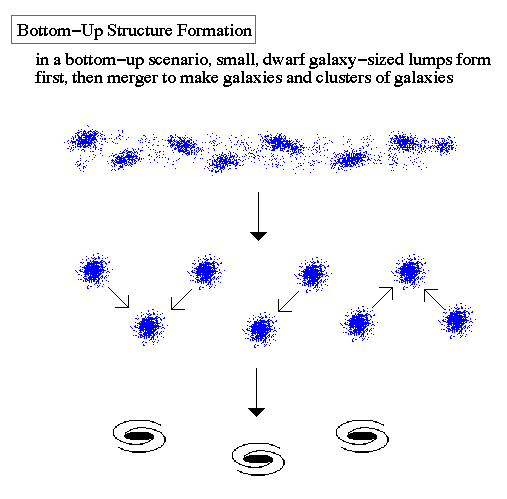
\includegraphics[width=0.5\columnwidth]{Visu/bottom_up.png}~%
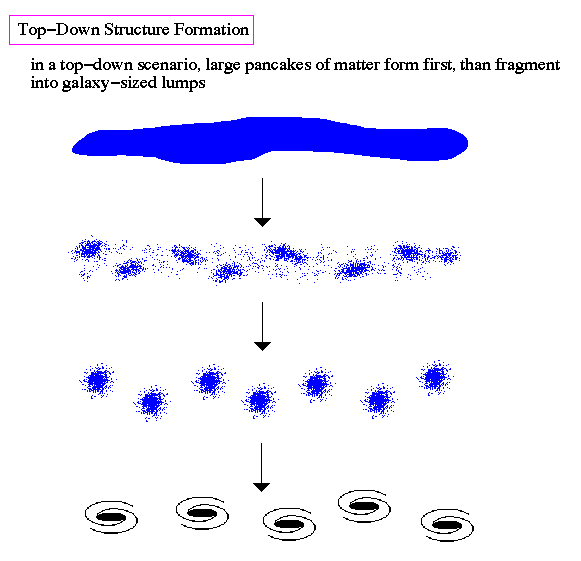
\includegraphics[width=0.5\columnwidth]{Visu/top_down.png}
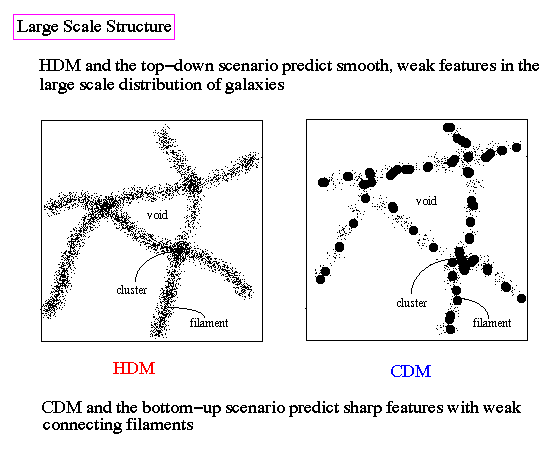
\includegraphics[width=0.75\columnwidth]{Visu/large_scale_structure.png}
\caption{Illustrations of the top-down and bottom-up structure formation. Credit: \url{http://abyss.uoregon.edu/~js/21st_century_science/lectures/lec27.html}}
\label{fig:lss_hdm_cdm}
\end{center}
\end{figure}

The equation of state for baryons is simply the squared sound velocity $\mathcal{P} = c^2_s \rho$, and the Jeans scale in Eq.~\ref{eq:damping_mode} with $w=c^2_s$ sets the critical regime whereabout modes larger or smaller than $k_{\mathrm{J}}/a$ will either oscillate (with a friction term in an expanding Universe) or grow exponentially. Indeed, the Jeans length is then the ratio between the gravitational dynamic time and the time scale of propagating pressure waves. This gravitational instability is at the heart of large scale structure formation. Depending on the order in which scales witness Jeans collapse, one can distinguish two broad scenarii of structure formation:\\

\begin{itemize}
\item[$\bullet$] \textbf{bottom-up}: structures of lower characteristic scales undergo gravitational collapse before coalescing into larger structures, illustrated in the left panel of Fig.~\ref{fig:lss_hdm_cdm};\\
\\
\item[$\bullet$] \textbf{top-down}: structures of larger characteristic scales undergo gravitational collapse before breaking apart into smaller structures, illustrated in the right panel of Fig.~\ref{fig:lss_hdm_cdm}.\\
\end{itemize}

In practice, the exact large scale structure formation may involve both scenarii. The characteristic of non-cold dark matter models is that large scales behave like pure CDM with a hierarchical structure formation, while smaller scales behave like hot dark matter, and involve the opposite scenario. The phenomenon responsible for this difference in behavior is the free-streaming  scale of the dark matter particles.

\subsubsection*{Collisionless Damping}


Contrary to the Jeans phenomenology, which applies to non-relativistic matter, the radiation populations (photons, hot dark matter, neutrinos) can free-stream out to a characteristic horizon without encountering any collisions. This collisionless damping \textit{a.k.a.} Landau damping \textit{a.k.a.} free streaming is characterized by an equation of state $w = \langle v^2_{\mathrm{th}} \rangle$ where $v_{\mathrm{th}}$ is the thermal velocity of the collisionless particle\\
\begin{equation}
\label{eq:thermal_velocity_mass}
\langle v_{\mathrm{th}} \rangle \simeq \left\{
\begin{array}{ll}
1 & \text{in the relativistic regime}\\
\\
\cfrac{\langle q \rangle}{m} \propto \cfrac{T}{m}& \text{in the non-relativistic regime}
\end{array}
\right.
\end{equation}\\

The Landau scale in the ultra-relativistic limit is simply the particle's causal horizon: $\lambda^{\mathrm{UR}}_{\mathrm{L}} \propto H^{-1}$. In the non-relativistic limit, the particle's  momentum decays like the background temperature and so the horizon scale is suppressed by the scale factor: $\lambda^{\mathrm{NR}}_{\mathrm{L}} \propto (aH)^{-1}$. Notice that in the infinitely massive limit, the Landau scale approaches zero $\lambda^{\mathrm{NR}}_{\mathrm{L}} (m \rightarrow \infty) \rightarrow 0$, which is expected for cold dark matter. \\

For particles becoming non-relativistic during the radiation dominated era,
$\lambda^{\mathrm{RDE}}_{\mathrm{L}} \propto t^{1/2}$ and so the comoving Landau scale $\lambda^{\mathrm{RDE}}_{\mathrm{L}}/a$ is constant. For particles becoming non-relativistic during the matter dominated era, the Landau scale $\lambda^{\mathrm{MDE}}_{\mathrm{L}} \propto t^{1/3}$ lengthens with time as expected, but slower than the Hubble radius and so the comoving Landau scale $\lambda^{\mathrm{MDE}}_{\mathrm{L}}/a \propto t^{-1/3}$ actually shrinks over time. Therefore, for particles becoming non-relativistic during the matter dominated era (which is the case for massive active neutrinos), $k_{\mathrm{L}}$ passes through a minimum at the time of transition, \textit{i.e.} when $m_\nu = \langle p_\nu \rangle = 3.15~ T_\nu$ which occurs at \\
\begin{equation}
a_{\mathrm{nr}}^{-1} = 1+z_{\mathrm{nr}} \simeq 2 \times 10^3 ~ \frac{m_\nu}{\mathrm{eV}}
\end{equation} \\ and so the mode of transition, corresponding to the maximum comoving free-streaming scale can be expressed as a function of $\omega_m = \Omega_m h^2$ and the neutrino's mass \\
\begin{equation}
\label{eq:knr}
k_{\mathrm{nr}} \simeq 0.018 ~\omega_m ~\frac{ m_\nu}{\mathrm{eV}}~\mathrm{Mpc}^{-1}
\end{equation}



\subsubsection{Hot Dark Matter}
\label{sec:hdm}

So far, the benchmark $\Lambda$CDM model has been consistently in adequation with nearly all cosmological observations. In CDM-based numerical simulations, the smallest structures collapse first and hierarchically coalesce into larger structures, in the so-called bottom-up scenario. It isn't, however, without its shortcomings. For one, in these purely cold dark matter simulations, the comoving numerical density of dark matter halos increases steeply at small masses: $dn/dM \propto M^{-1.9}$ and consequently yield many more small dark matter halos than larger ones. Hundreds of $\sim 10^{8}M_{\odot}$ sub-halos are predicted in the vicinity of the Milky Way, whereas only a handful have been observed. This may be due to the challenge posed by observing dark matter rich halos, as it is unclear whether tracers such as stars and gas populate lighter halos as heavier ones. Furthermore, it has been shown that baryonic processes and non-linear feedback mechanisms can alter the predicted number of small mass halos to some degree. Another issue is that CDM predicts cuspy density profiles of individual halos, \textit{i.e.} a monotonically increasing density profile at small radii. The observed density profiles of dark matter halos caps at a core value, making them less ``cuspy'' than the prediction. Here again, baryonic processes may play an essential yet non-trivial role in this discrepency.\\

\begin{figure}
\begin{center}
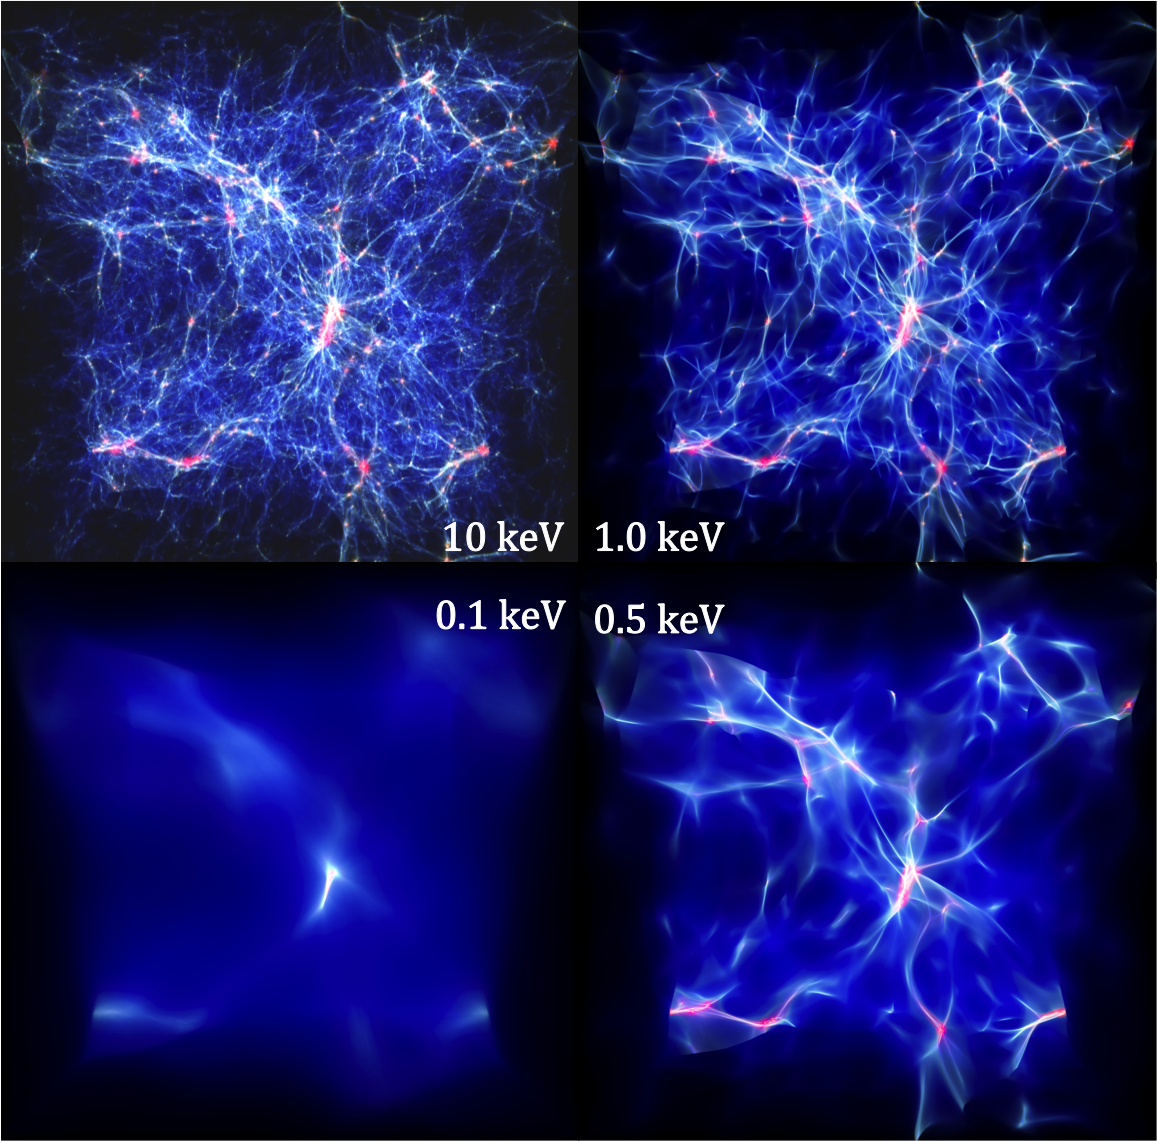
\includegraphics[width=\columnwidth]{Visu/CWH.png}
\caption{Distribution of $768^3$ baryon gas particles in a comoving volume of $(25~h^{-1}\mathrm{Mpc})^3$ with differing mass for the dark matter particle, listed in the corner of the panels. The snapshot images are realized using the \texttt{Splotch} software; Temperature is represented by the color palette while the intensity denotes gas density. The top two panels with $m_{\mathrm{dm}} \gtrsim 1 ~\mathrm{keV}$ are considered warm dark matter, with the top left one being visually indistinguishable from standard CDM (infinite mass limit). The bottom two panels with $m_{\mathrm{dm}} \lesssim 1 ~\mathrm{keV}$ are considered hot dark matter and violate the Tremaine-Gunn bound.}
\label{fig:visu_wdm}
\end{center}
\end{figure}

Nevertheless, these ``cuspy core'' and ``low satellite count'' issues can both be accounted for if one assumes the dark matter candidate particle has a wider velocity dispersion than the CDM velocity distribution which is ideally as narrow as can be. These non-cold dark matter models involve additional parameters, the most relevant being the mass of the particle which determines its thermal velocity and hence its free-streaming horizon. Fig.~\ref{fig:visu_wdm} features the distribution of baryon gas (tracing the dark matter distribution) in a comoving volume of one of the hydrodynamics simulations I performed (see Chap.~\ref{chap:Simulations}) with different values of the dark matter particle mass. Predictably, according to Eq.~\ref{eq:thermal_velocity_mass} and Eq.~\ref{eq:damping_scale}, as the DM particle mass decreases, the free-streaming damping scale increases. As a result, smaller-mass structures in pure hot dark matter models (in which $m_{\mathrm{hdm}} \lesssim 1 ~\mathrm{keV}$) fragment from heavier and larger structures in a top-down structure formation scenario. As a result, structures on the smallest scales end up forming considerably later than in the standard CDM case, which is manifest as a cutoff in the matter power spectrum in Fig.~\ref{fig:initialpwrspc}. \\

Similarly to the CDM transfer function, it is useful to define a NCDM (here, pure HDM) matter transfer function $T_m(k, z)$, which is defined as\\
\begin{align}
P_m(k) &= \left\langle \left\vert \frac{\sum\limits_{\alpha \in m} \delta \rho_\alpha}{\sum\limits_{\alpha \in m} \rho_\alpha} \right\vert^2 \right\rangle \\
&= \left\langle \left\vert \frac{\sum\limits_{\alpha \in m} \delta_\alpha \Omega_\alpha}{\sum\limits_{\alpha \in m} \Omega_\alpha} \right\vert^2 \right\rangle \\
&= T^2_m (k) \times \left\langle \left\vert \delta_{\mathrm{cdm}} \right\vert^2 \right\rangle \\
&= T^2_m (k) \times P_{\mathrm{cdm}} (k)
\end{align} \\ where $P_{\mathrm{cdm}}$ is given by Eq.~\ref{def:cdm_tf}. Fig.~\ref{fig:pk_wdm} features the hot and warm (see Sec.~\ref{sec:warmy} for distinction) dark matter transfer function (squared), which can be approximated by the analytical fit \citep{Bode2000}\\
\begin{equation}
\label{eq:fit}
T(k, z=0) \simeq \left( \frac{1}{1 + \left( \beta~k \right)^{2 \gamma}} \right)^{\gamma/5}
\end{equation} \\ in which \cite{VLH08a} find $\gamma = 1.12$; and the breaking scale is a function of mass:\\
\begin{equation}
\beta = 0.24 \left( \frac{1}{\alpha} \frac{\mathrm{keV}}{m_x} \right)^{0.83} \left( \frac{\omega_x}{0.25 \times 0.7^2} \right)^{-0.16}~\mathrm{Mpc}
\end{equation} \\ with $m_x$ the mass assuming the particle is an early-decoupled thermal relic of temperature $T_x = \alpha T_\nu$, and $\omega_x = \Omega_x h^2 = \omega_{\mathrm{dm}}$. Those values best fitted by \cite{VLH08a} are only valid for scales $k \leqslant 5~h~\mathrm{Mpc}^{-1}$. \\

Ever since the advent of numerical cosmological simulations in the early 1980's, neutrinos were implemented as the dark matter, since they were at the time the only viable candidate in existence. As apparent from Eq.~\ref{eq:knr}, a $\sim \mathrm{eV}$ neutrino free-streams up to $\sim 40$ comoving Mpc, which is several tens of times the extent of a typical galaxy. If neutrinos were the dark matter, then galaxy formation would be delayed until late cosmological times, as was also deduced from the early numerical simulations. High redshift quasars, which are hosted by galaxies, represent direct evidence against this scenario. This means that the 3 lepton-flavored $\lesssim \mathrm{eV}$ neutrinos cannot account for the entirety of dark matter. Either they are only partially so, which I explore in Sec.~\ref{sec:mdmps}, or neutrinos are much more massive than the electron-volt scale. If neutrinos consititute the dark matter, then it can only be a heavier neutrino mass eigenstate whose existence has yet to be confirmed. Of course, other theoretical particles other than neutrinos can be an adequate pure dark matter candidate, so long as its mass is heavy enough so that its free-streaming horizon does not damp out galactic (and sub-galactic) sized structures. This is what is still currently under investigation since the early 2000's, which I lay out in Sec.~\ref{sec:warmy}.


\subsubsection{Warm Dark Matter}
\label{sec:warmy}

Not only are $\sim \mathrm{eV}$ scale particles including left-handed neutrinos unviable DM candidates, so is any fermion lighter than $\sim 0.5~\mathrm{keV}$. This is known as the Tremaine-Gunn bound \citep{Tremaine-Gunn}, which poses that the average phase-space density distribution $\bar{f}$ of a fermionic DM particle in a DM-rich system --- such as a dwarf spheroidal galaxy satellite --- be greater than the phase-space density of a degenerate Fermi gas. A similar although stronger bound exists for bosonic dark matter, which can be derived from the Liouville theorem. The distinction between hot and warm dark matter conventionally occurs at this critical limit. Although HDM is empirically excluded, fermions heavier than $\sim 0.5~\mathrm{keV}$ can be a WDM candidate, such as the right-handed neutrino introduced by \cite{DodelsonWidrow94}. Their free-streaming horizon is shorter than that of left-handed neutrinos by the same $10^3$ factor, and as such are at the goldilocks zone in terms of dark matter properties: they are light (hot) enough to damp small scale structures and thus circumvent the cuspy core and galaxy sattelite count issues; all-the-while heavy (cold) enough so that large-scale structures are virtually unaffected by their free-streaming and are indistinguishable from CDM. The top two panels of Fig.~\ref{fig:visu_wdm} illustrate this dual behavior: CDM-like at large scales while HDM-like at small scales. This is quantified in the warm to cold dark matter transfer function $T$ displayed in Fig.~\ref{fig:pk_wdm}, where the WDM power spectrum is indistinguishable from the CDM one for low values of $k$. The cutoff materializes the free-streaming horizon, which occurs at larger values of $k$ as $m$ increases. As such, the heavier (colder) the WDM particle, the more compatible with CDM and observations. Fig.~\ref{fig:pk_wdm} also shows that kilo-$\mathrm{eV}$ WDM particles can be probed by the Lyman-alpha forests power spectrum, which is the main observable of my work, and which integrates power along $k_\parallel$ from $k$ scales greater than that denoted by the vertical black line to $k \rightarrow \infty$.  \\


\begin{figure}
\begin{center}
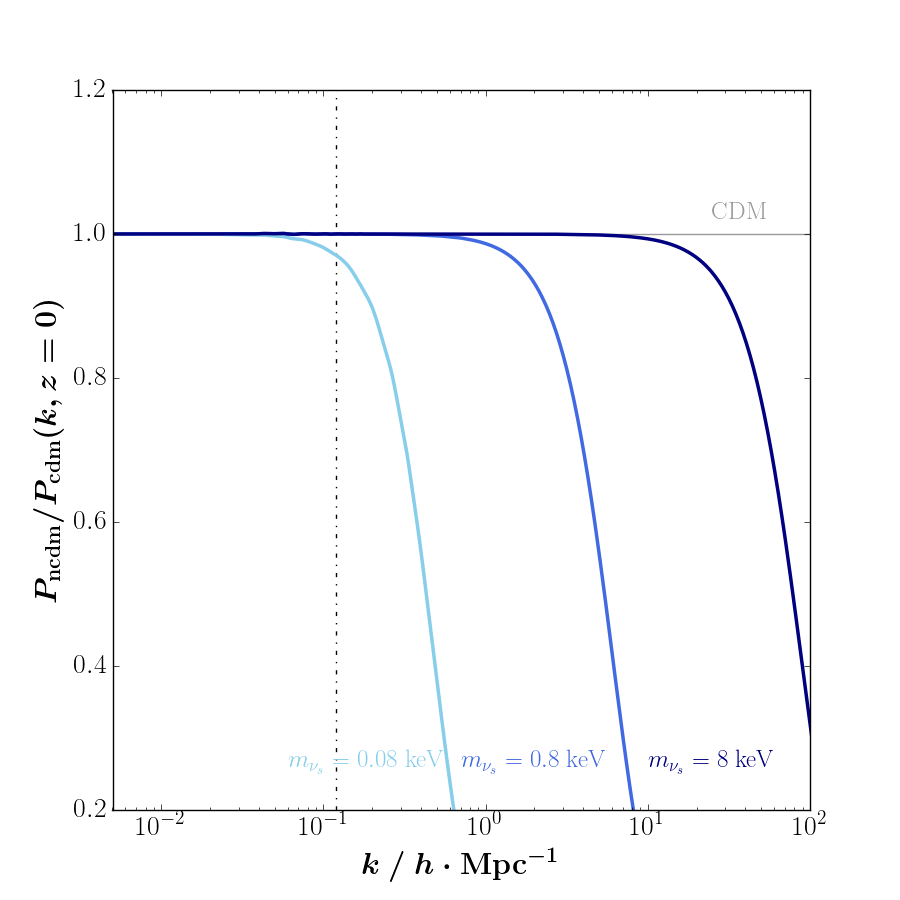
\includegraphics[width=0.75\columnwidth]{Pk_wdm.png}
\caption{Matter power spectrum at $z=0$ in a pure WDM cosmology, normalized by that of the benchmark CDM model, for $m_{\nu_s} = 8 \times 10^{-2, -1, 0}\mathrm{keV}$. The vertical dot-dashed line signals the lowest $k$ probed by Lyman-alpha forests.}
\label{fig:pk_wdm}
\end{center}
\end{figure}

As introduced in the above discussions, when particles have relativistic enough velocities, they free-stream to a horizon scale $\lambda_{\rm{FSH}}$ effectively unaffected by gravitational potentials. The matter power spectrum is suppressed below the free-streaming horizon, which is given by 
\begin{empheq}[box=\mymath]{equation}
\lambda_{\mathrm{FSH}}(t) = a(t) \int_0^{a(t)} da \frac{\langle v \rangle}{a^2 H}
\end{empheq}
where the velocity dispersion $\langle v \rangle$ is given by the speed of light during the relativistic regime, and by  ${\langle p \rangle}/{m}$ afterwards. For warm and cool dark matter, this transition takes place during the radiation dominated era. The associated comoving scale
\begin{equation}
\frac{\lambda_{\mathrm{FSH}}(t)}{a(t)} = \frac{2 \pi}{k_{\mathrm{FSH}}(t)}
\end{equation}
grows like $t^{1/2}$ during the relativistic regime, like $\ln(t)$ during the non-relativistic regime as long as radiation dominates, and remains asymptotically constant during matter domination. Finally the comoving free-streaming horizon today can be estimated from
\begin{equation}
\frac{\lambda_{\mathrm{FSH}}^0}{a_0} = \frac{2 \pi}{k_{\mathrm{FSH}}^0}
\simeq \int_0^{a_{\rm{nr}}} \frac{da}{a^2 H} +  \int_{a_{\rm{nr}}}^{a_0} \frac{a_{\rm{nr}} da}{a^3 H}~,
\label{eq:FSH_L}
\end{equation}
where $a_{\rm{nr}} \simeq {\langle p \rangle_0}/{m}$ is the scale factor at
the time of the non-relativistic transition, and $\langle p \rangle_0$ is the
momentum dispersion today. Distant quasars probe the power spectrum at scales of several Mpc. They enable putting upper bounds on $k_{\rm{FSH}}^0$ of keV NCDM particles, which translate into lower bounds on their mass. The velocity and momentum dispersion requires knowledge of the explicit distribution function of the particle, which differs from a Fermi-Dirac (thermal) distribution function depending on the production mechanism. Thus \emph{the mass bounds are different for each production mechanism}. \\


\subsubsection*{Early Decoupled Thermal Relics}

In Sec.~\ref{sec:extrarad}, I introduced early-decoupled thermal relics, which are essentially thermalized particles that decouple deep within the radiation dominated era while relativistic. Thermal relics of masses of a few keV are ideal warm dark matter candidates, and include gravitinos, neutralinos and other Weakly Interacting Massive particles (WIMPs). If they make up the entirety of the dark matter population, then \\
\begin{equation}
\left\{ 
\begin{array}{l}
\Omega_x h^2 = \cfrac{m_\nu^{\mathrm{eff}}}{93.14~ \mathrm{eV}} \\
\Delta N_{\mathrm{eff}} = \left( \cfrac{m_\nu^{\mathrm{eff}}}{m_x} \right)^{4/3} = \left( \cfrac{T_x}{T_\nu} \right)^4
\end{array}
\right.
\end{equation} \\ Since their momenta are distributed according to a Fermi function, a code like \texttt{CAMB} can straightforwardly account for such a dark matter particle by setting $\Omega_{\mathrm{cdm}} = 0$, $\Omega_\nu = \Omega_x$, and incorporate the mass and temperature of the thermal relic in $\Delta N_{\mathrm{eff}}$ which can be set via the \texttt{nu\_mass\_degeneracies} input parameter. Tab.~\ref{tab:camb_param} in Sec.~\ref{sec:ips} recaps all the input paramaters for the \texttt{CAMB} software I use to model neutrinos and, in this specific case, thermal relic dark matter. I check that this procedure reproduces the results from \cite{VLH08a} on the linear matter transfer function. In Fig.~\ref{fig:pk_lin_x}, I show the outputs of 5 thermal relics as warm dark matter candidates at $z=2.5$, along with the numerical fit from Eq.~\ref{eq:fit}, which bears resemblance to Fig.~1 in \cite{VLH08a}. \\


\begin{figure}
\begin{center}
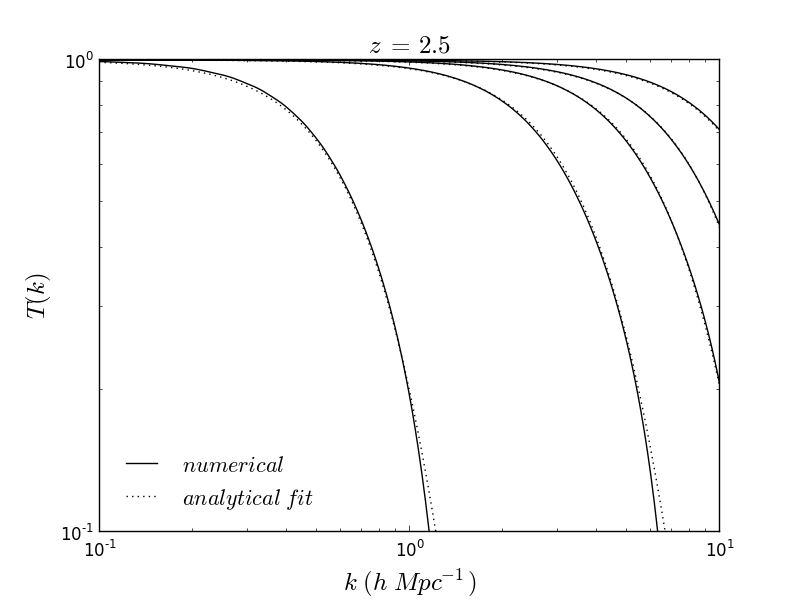
\includegraphics[width=0.75\columnwidth]{CC/camb__transfer_test.png}
\caption{Linear matter transfer function at $z=2.5$ for 5 pure WDM models assuming $\Omega_b=0.05$, $\Omega_{\mathrm{dm}} = 0.25$ and $\Omega_\Lambda = 0.7$. The solid curves labelled `numerical' correspond to a thermal relic of (left to right) $T_x/T_\nu = 0.5, 0.3, 0.25, 0.226$ and $0.2$, or equivalently, $m_x/\mathrm{keV} = 0.092, 0.427, 0.728, 1.000$ and $1.441$ respectively, produced with \texttt{CAMB}. The dotted lines labelled `analytical fit' are from Eq.~\ref{eq:fit}.}
\label{fig:pk_lin_x}
\end{center}
\end{figure}


\subsubsection*{Non-Resonantly Produced Right-Handed Neutrinos}

Sterile neutrino were originally proposed as dark matter candidates by \cite{DodelsonWidrow94}, `DW' herein.  In the framework of DW, sterile neutrinos are predominantly produced  at 
$T \sim 150~\mathrm{MeV}(m_{\nu_s}/\mathrm{keV})^{1/3}$ when the oscillation production
rate is most efficient while not reaching thermal
equilibrium~\citep{DodelsonWidrow94, Dolgov2000ew, Abazajian2001nj, Asaka2006nq}.  The resulting distribution
function can be roughly approximated by a rescaled Fermi-Dirac
distribution~\citep{Dolgov2000ew}, in which case the average momentum
$\langle p\rangle$ would be identical to that of active neutrinos. The
proper treatment however, based on the quantum Liouville equation~\citep{Asaka2006rw}
shows that sterile neutrinos produced in (non-resonant) oscillations do not
feature a re-scaled thermal distribution and their average momentum is about 10--40\% colder
depending on sterile neutrino mass (see Fig.~8 in~\cite{Asaka2006nq} or
Fig.~6 in~\cite{Laine2008pg}). To distinguish them from the idealized DW
case, I refer to sterile neutrinos produced via this mechanism as \emph{non-resonant} (see Sec.~\ref{sec:rhneu} for distinction), or NRP sterile neutrinos. \\


The requirement  $\Omega_{\nu_s} = \Omega_{\rm{dm}}$ fixes the $\theta$ --
$m_{\nu_s}^{\rm{nrp}}$ relationship, represented as the upper black solid line
in Fig.~\ref{fig:RPSN_MT}. The flux of photons from the radiative decay channel
$\nu_s \rightarrow \gamma \nu_\alpha$ is a function of $\theta$ and
$m_{\nu_s}$~\citep{Pal1981rm}. Decay lines in astrophysical spectra, or the
lack thereof, thus establishes constraints on these
parameters, see~\cite{Dolgov2000ew, Abazajian2001vt, Boyarsky2005us, Boyarsky2006fg}. Comparing
the upper bounds on the putative dark matter decay flux with currently measured  DM abundance, \cite{BNRST06} and \cite{BNR07} yield an upper limit of $m_{\nu_s}^{\rm{nrp}} \leq 4~\rm{keV}$ for the NRP mechanism. The non-detection of small-scale damping in the flux power spectrum of the Ly-$\alpha$ forest due to $\nu_s$ free-streaming has yielded lower bounds consistently above the $4~\rm{keV}$ limit with $\geq 5 \sigma$ (see Tab.~\ref{tab:studies} in Sec.~\ref{sec:pureWDM}). If right-handed neutrinos constitute all of dark matter, a growing consensus suggests they cannot be produced in this oscillation mechanism in absence of a net lepton asymmetry.


\subsubsection{Cool Dark Matter}
\label{sec:rpsn_intro}

The presence of a net lepton asymmetry at temperatures $T \sim 0.1~\rm{GeV}$
can significantly enhance the production of sterile neutrinos from active
neutrinos through forward scattering in dense media \citep{ShiFuller99}. In a mechanism similar to the MSW\footnote{Mikheyev-Smirnov-Wolfenstein} effect~\citep{Mikheev1986gs, Wolfenstein1977ue} accounting for the solar neutrino deficit, the excessive abundance of leptons and their conjugate neutrinos with respect to anti-leptons can yield the correct DM density $\Omega_{\rm{dm}}$ with weaker mixing angles $\theta$. \cite{ShiFuller99} showed that this resonant production (RP) yields sterile neutrinos with significantly cooler momenta than the NRP ones. The resonant momenta depend on the sterile neutrino mass $m_{\nu_s}^{\rm{rp}}$ and net leptonic (assumed electronic) asymmetry $\mathcal{L} = (n_{\nu_e} - n_{\bar{\nu}_e}) / s$ in units of entropy density where $s \propto g_\star T^3$. If the resonance occurs before the QCD phase transition, only the low momenta states are populated from the quasi thermally-distributed active neutrinos ($\langle q = p/T_\nu \rangle \simeq 3.15$), resulting in cooler neutrino and anti-neutrino distribution functions with $\langle q \rangle \simeq 1.6$. \\

The left panel in Fig.~\ref{fig:M4L12_fs} features the distribution functions of $m_{\nu_s} = 4~\mathrm{keV}$ sterile neutrinos, one (in grey) non-resonantly produced, \textit{i.e.} in absence of lepton asymetry, and the other with $\vert n_{\nu_e} - n_{\bar{\nu}_e} \vert / s = \mathcal{L} = 1.2 \times 10^{-5}$ which yields the coolest distribution function for this mass. Producing such phase-space distribution (PSD) functions requires a dedicated software that solves the Boltzmann equation (see Eq.~\ref{eq:Merle}) for both the sterile neutrino and its associated anti-neutrino. While investigating this line of research, I tried to produce the PSD with the public code \texttt{sterile-dm}\footnote{\url{https://github.com/ntveem/sterile-dm}} by \cite{sterile-dm}. I was unsuccessful in reproducing Fig.~2 of \cite{Abazajian2014} in producing the PSD for a $m_{\nu_s} = 7.14~ \mathrm{keV}$ sterile neutrino with 5 lepton asymmetry parameters. The reason for which I was unsuccessful is that I was unable to run the code for a given RPSN model with $\left( m_{\nu_s}, \mathcal{L} \right)$ for a fixed value of $\omega_{\mathrm{dm}}$. The code yields the resulting value of the lepton asymmetry from the value of the active-sterile mixing angle $\theta$. There is no analytical relationship between $\theta$ and $\mathcal{L}$. To remedy this, I ran the code on a $50 \times 50$ uniform grid of $\log_{10} \left( \sin^2 2 \theta \right)$ and $\log_{10} \left( m_{\nu_s} / \mathrm{keV} \right)$ with $\omega_{\mathrm{dm}} = 0.1185$ and report the resulting values of the lepton asymmetry in the right panel of Fig.~\ref{fig:rpsn_steriledm_7keV}. Not only was the code not able to converge for certain input values, visible as horizontal white stripes and checkers on the right-hand side of the parameter space, but even for values on which it converged, the resulting value of $\Omega_{\mathrm{dm}}$ was to far off of what was initially set. This is not to say that the code is troublesome. In fact, it solves the Boltzmann function very accurately by taking into account a number of subtle thermodynamic phase transitions in the early Universe, and is considered by many as the state-of-the-art in terms of producing accurate PSDs for RPSN. I did not benefit of enough time to familiarize myself with the inner workings of the code, and decided to try another route. I do, however, recommend this code for any future investigation. \\


\begin{figure}
\begin{center}
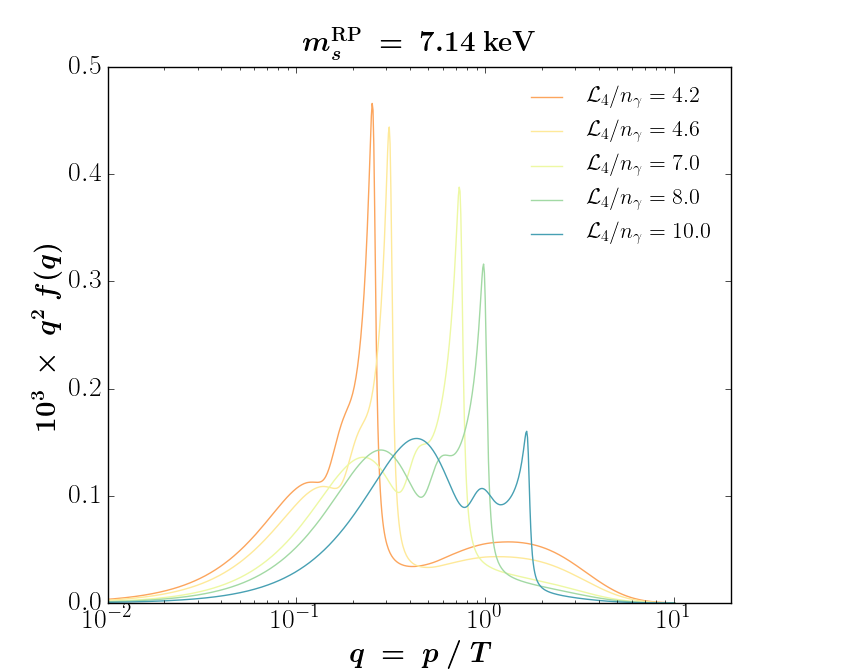
\includegraphics[width=0.55\columnwidth]{RPSN/M7keV_Aba_zoom.png}~%
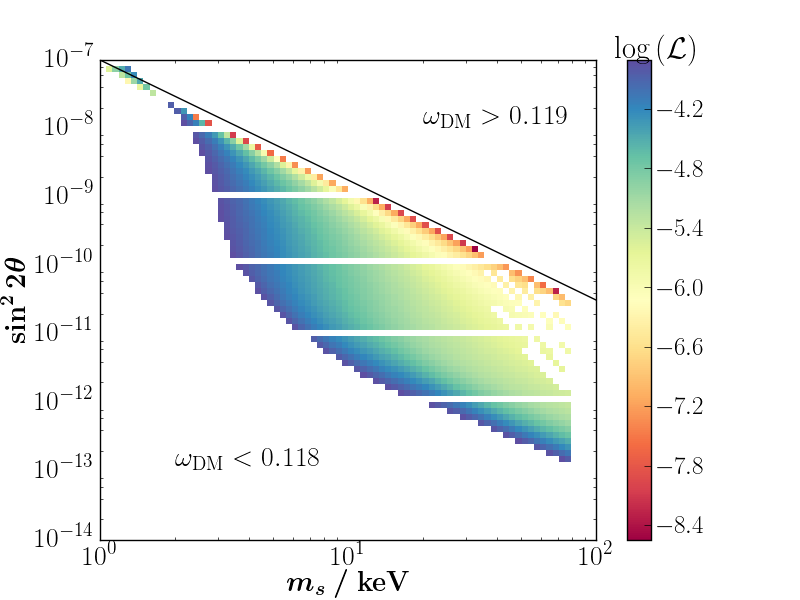
\includegraphics[width=0.55\columnwidth]{RPSN/Lgrid_fit_emp.png}
\caption{\textbf{Left:} PSD of 5 RPSN models as pure cool dark matter assuming $\omega_\mathrm{dm} = 0.1185$, for $10^4~\mathcal{L} / n_\gamma = 4.2, 4.6, 7, 8$ and $10$. These values are chosen to attempt reproducing Fig.~2 of \cite{Abazajian2014}, with adapted definition of the lepton asymmetry parameter. \textbf{Right:} Value of $\mathcal{L}$ as a function of the mixing angle and RPSN mass, using the \texttt{sterile-dm} code. The black solid line corresponds to the Dodelson Widrow mechanism.}
\label{fig:rpsn_steriledm_7keV}
\end{center}
\end{figure}

I initiated a collaboration with a team of international researchers\footnote{Julien Lesgourgues (TTK -- Aachen), Oleg Ruchayskiy (Niels Bohr Insitute -- Copenhagen) and Alexey Boyarksy (Lorentz Institute -- Leiden)} that are exterior to our group. Using a Boltzmann solver code described in \cite{LaineMSM, Ghiglieri2015jua}, we were able to produce the distribution functions for $16$ masses $m_{\nu_s} = 1~\mathrm{keV}$ to $m_{\nu_s} = 19~\mathrm{keV}$ with step $\Delta m_{\nu_s} = 1~\mathrm{keV}$ excluding $12, 15$ and $18~\mathrm{keV}$; each for $30$ uniformely increasing values of $\mathcal{L}_6 \doteq \mathcal{L} / 10^{-6}$ of step $\Delta \mathcal{L}_6 = 1$ from $\mathcal{L}_6 = 0$ to $25$, in addition to $\mathcal{L}_6 = 50, 100, 120$ and $700$. I display in Fig.~\ref{fig:rpsn_banana} the value of $\langle q
\rangle / m_{\nu_s}$ for the entire grid of $16 \times 30$ RPSN distribution functions at our disposal, all computed using the code descibed in \cite{LaineMSM, Ghiglieri2015jua}. The coolest distribution functions occur for given values of $\mathcal{L}$ and $m_{\nu_s}^{\rm{rp}}$, which I denote $\mathcal{L}^{\star} (m_{\nu_s})$. For larger asymmetries than $\mathcal{L}^{\star}$ for a given mass, the resonantly boosted forward scattering occurs later than the QCD phase transition, which yield quasi-Fermi populated momenta states (with weaker mixing angles). \\

\begin{figure}
\begin{center}
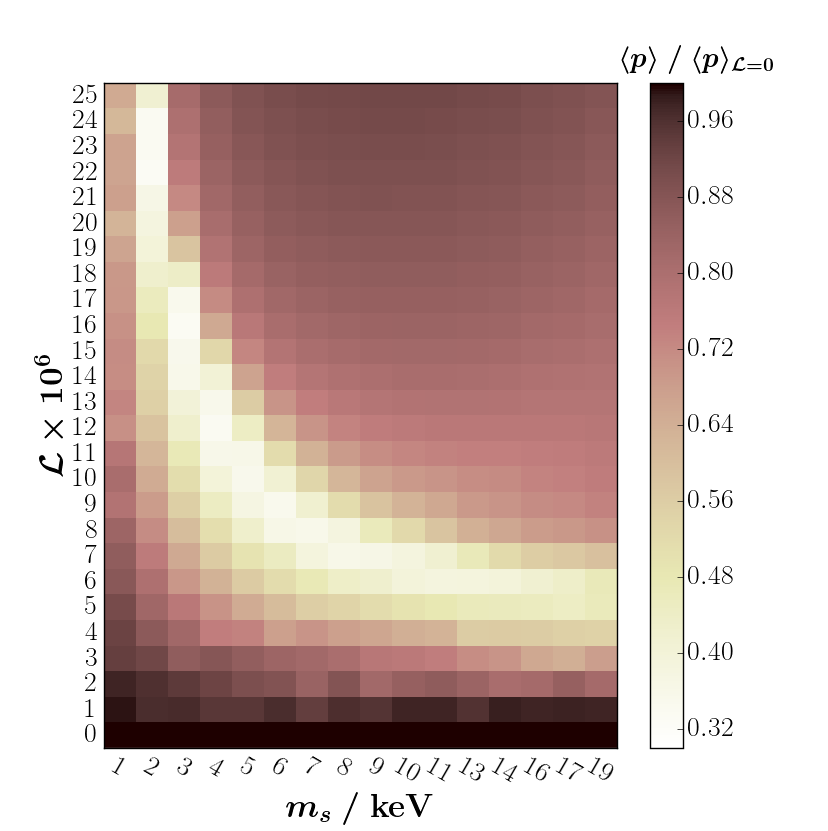
\includegraphics[width=0.8\columnwidth]{RPSN/RPSN_mean_momentum.png}
\caption{Average momentum per mass
  $\langle q \rangle / m_{\nu_s}$ of the RPSN distribution functions computed in \cite{LaineMSM} and normalised to the NRP ($\mathcal{L}=0$) case for each mass (bottom-most row). Lepton asymmetries are in units of
  $\mathcal L = \left( n_{\nu_e} - n_{\bar{\nu}_{e}} \right) / s$. For each
  mass, the value of $\mathcal{L}^{\star}$ yielding the coolest distribution
  function is easily identifiable.}
\label{fig:rpsn_banana}
\end{center}
\end{figure}

These PSD are then passed down to the \texttt{CLASS} software (see Sec.~\ref{sec:ips}) which computes the linear matter transfer function from the PSD. This not only enables us to test pure cool dark matter cosmologies with a set of RPSN models, which I enumerate in List~\ref{eq:RPSN_models_simu}, but also constrain the entire relevant $\left( m_{\nu_s}, \mathcal{L} \right)$ parameter space using a mapping procedure with C+WDM models, which I describe in Sec.~\ref{sec:map_rpsn_cwdm}.


%%%%%%%%%%%%%%%%%%%%%%%%%%%%%%%%%%%%%%%%%%%%%%%%%%%%%
\subsection{Power Spectrum of Mixed Dark Matter}
%%%%%%%%%%%%%%%%%%%%%%%%%%%%%%%%%%%%%%%%%%%%%%%%%%%%%
\label{sec:mdmps}

In Sec.~\ref{sec:hdm}, I exposed the arguments that made standard model neutrinos unable to account for all of dark matter. This isn't to say that neutrinos aren't a dark matter candidate, but rather that if dark matter is made up of particles, then only a portion of the total population can be neutrinos, or else dark matter would have free-streamed out to intergalactic scales, washing away any perturbations smaller than these wavelengths. The relevant question is how much of dark matter do neutrinos make up ? In this section, I assume that dark matter is bi-phasal: \\

\begin{itemize}

\item[$\bullet$] a non-cold component of relative abundance $0 \leqslant F \leqslant 1$ \\

\item[$\bullet$] a cold component of relative abundance $1 - F$ \\

\end{itemize}

In this framework, the non-cold to total dark matter ration $F$ constitutes an additional free parameter to the cosmological model. It interpolates between the pure cold dark matter ($F = 0$) and the pure hot dark matter ($F = 1$) limit cases. In what follows, I show how this parameter impacts the linear power spectrum. First, in Sec.~\ref{sec:chdm_sub}, I assume the non-cold component is made of a generic hot dark matter particle, such as active neutrinos. Then, in Sec.~\ref{sec:cwdm_linear}, I assume the non-cold component is a generic warm (or cool) dark matter particle, such as early decoupled thermal relics and sterile neutrinos. 

\subsubsection{Cold+Hot Dark Matter}
\label{sec:chdm_sub}

The free-streaming of neutrinos never impacts scales beyond the non-relativistic transition ($k < k_{\mathrm{nr}}$). In the non-relativistic regime, neutrinos are essentially indistinguishable from cold dark matter and the background evolution. The large-scale portion of the power spectrum is thus insensitive to the neutrino masses. On the other hand, neutrino power is depleted on scales within the free-streaming horizon ($k \geqslant k_{\mathrm{nr}}$) by a factor $\delta_\nu / \delta_{\mathrm{cdm}}$ which reaches $0$ in the $k \rightarrow \infty$ limit. The asymptotical behavior of the matter transfer function is thus \\
\begin{equation}
T^2_m (k) \simeq \left\{
\begin{array}{ccl}
1 & \text{for} & k < k_{\mathrm{nr}}\\
(1-f_\nu)^2 & \text{for} & k \gg k_{\mathrm{nr}}
\end{array}
\right.
\end{equation} \\ where the neutrino abundance parameter $f_\nu$ is defined as \\
\begin{empheq}[box=\mymath]{equation}
\label{eq:f_nu}
f_\nu = \frac{\rho_\nu}{\rho_\nu + \rho_b + \rho_{\mathrm{cdm}}} = \frac{\Omega_\nu}{\Omega_m}
\end{empheq}

\begin{figure}
\begin{center}
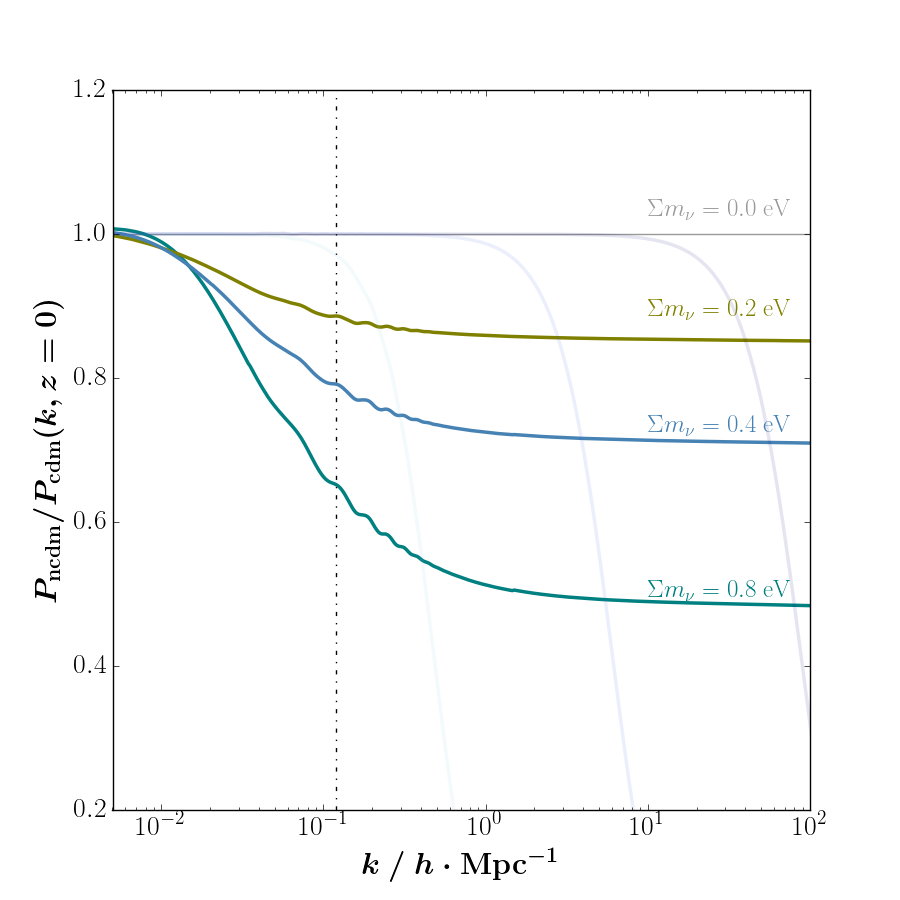
\includegraphics[width=0.75\columnwidth]{Pk_chdm.png}
\caption{Matter power spectrum at $z=0$ in a mixed C+HDM cosmology, normalized by that of the benchmark CDM model, for $\sum m_\nu = 0.2, 0.4, 0.8~\mathrm{eV}$. The vertical dot-dashed line signals the lowest $k$ probed by Lyman-alpha forests. The matter power spectra of pure WDM displayed in Fig.~\ref{fig:pk_wdm} are superimposed in light grey for comparative purposes.}
\label{fig:pk_chdm}
\end{center}
\end{figure}


The depletion factor of neutrinos within their free-streaming horizon is not exactly the $f_\nu$ factor in the above expression since neutrino density contrasts issue back-reactions on the evolution of the metric and on all other perturbations. $\delta_\nu$ does not contribute significantly to the Poisson equation, however $\bar{\rho}_\nu$ (assumed to be dominated by non-relativistic neutrinos) fixes the expansion rate via the Friedmann equation \\
\begin{equation}
3 \left( \frac{\dot{a}}{a} \right)^2 = 8 \pi G a^2 \left( \bar{\rho}_\nu + \bar{\rho}_b + \bar{\rho}_{\mathrm{cdm}} \right)
\end{equation} During the Radiation Dominated Era, the scale factor evolves as $a \propto \tau^2$ and so\\
\begin{equation}
\ddot{\delta}_{\mathrm{cdm}} + \frac{2}{\tau} \dot{\delta}_{\mathrm{cdm}} - \frac{6}{\tau^2} (1-f_\nu) \delta_{\mathrm{cdm}} = 0
\end{equation} \\ the growing solution of which is \\
\begin{equation}
\delta_{\mathrm{cdm}} \propto a^{1-\frac{3}{5}~f_\nu}
\end{equation} \\ if $f_\nu \ll 1$. Given the time during which the growth is suppressed by the $3/5~f_\nu$ factor, \textit{i.e.} until neutrinos become non-relativistic, \cite{LESGOURGUES2006} show that the impact on the matter power spectrum can be approximated by \\
\begin{equation}
\label{eq:tnu}
\frac{\Delta P_m}{P_m} \simeq - 8 f_\nu
\end{equation} \\ It turns out that the factor is actually closer to $- 10 f_{\nu}$ when accounting for non-linear effects. \\

The neutrino density is fixed by the effective mass parameter $m_\nu^{\mathrm{eff}}$ which is $N_\nu m_\nu$ in the case of $N_\nu \simeq 3$ degenerate neutrino mass eigenstates $m_\nu$. In practice, we are sensitive only to the sum mass $\sum m_\nu$ and so\\
 
\begin{equation}
\label{eq:meff_link}
\omega_\nu = \frac{m_\nu^{\mathrm{eff}}}{93.14~\mathrm{eV}} = \frac{\sum m_\nu}{93.14~\mathrm{eV}} = \frac{N_\nu m_\nu}{93.14~\mathrm{eV}}
\end{equation} \\

Hence the relative suppression in power can be expressed as a linear function of the effective neutrino mass in the eV and the sub-eV regime:\\

\begin{equation}
\frac{\Delta P_m}{P_m} \simeq - 10\frac{\Omega_\nu}{\Omega_m} \simeq - 0.1 \frac{m_\nu}{\mathrm{eV}} \frac{N_\nu}{\Omega_m h^2}
\end{equation}


\subsubsection{Impact of Mass Ordering}
\label{sec:mass_ordering}

\begin{figure}
\begin{center}
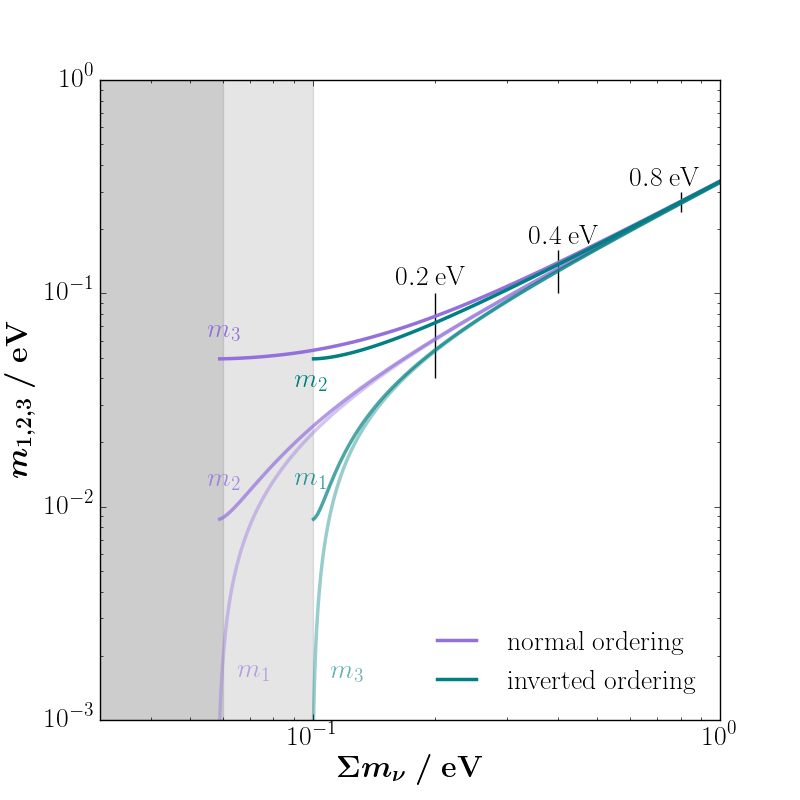
\includegraphics[width=0.8\columnwidth]{Smnu_mnu.png}
\caption{Values of the individual mass eigenstates $m_1, m_2, m_3$ in $\mathrm{eV}$ as a function of $\sum m_\nu = m_1 + m_2 + m_3$ in the `normal' (lavender) and `inverted' (teal) mass orderings. $m_3$ vanishes to a massless eigenstate below $\sum m_\nu \leq 0.10~(0.06)~~\mathrm{eV}$ in the inverted (\textit{resp.} normal) configuration. Above $\sum m_\nu \gtrsim 0.4~\mathrm{eV}$, the two mass orderings are barely distinguishable from the `degenerate' configuration in which $m_1 = m_2 = m_3$.}
\label{fig:smnu_mnu}
\end{center}
\end{figure}

Cosmology is mainly sensitive to neutrino masses through their contribution to the energy density, \textit{i.e.}, through $\Omega_\nu$, and therefore only through the total mass of the eigenstates $\sum m_\nu$. While this is true to a very good approximation for the CMB anisotropy spectrum, the impact of individual neutrino masses on Large Scale Structures can issue some subtlety. Although  the main effect remains that of the total mass, matter power spectrum measurements have some  sensitivity to individual eigenstate masses because of two effects:  \\
\begin{itemize}
\item[$\bullet$] the detailed evolution of the background density close to the time of the non-relativistic transition of each species depends on individual masses; \\
\item[$\bullet$] and so does the free-streaming scale of each species.\\
\end{itemize}
In practice, it is the lepton flavor of neutrinos which differentiates them, each flavor state being a superposition of oscillating mass eigenstates. Here, I only regard the propagation fo the mass eigenstates --- which is what I refer to as the \emph{individual} masses --- and the relative difference between them through neutrino oscillations, not the mass of the flavor states which are composite. When the individual masses are varied for the same total mass, the two effects listed above lead respectively to different amplitude and shape in the small-scale portion of the matter power spectrum~\citep{Lesgourgues2006nd, Lesgourgues2013neutrino}. \\

Throughout this work as well as what was accomplished before I was integrated in this project, we assumed the three neutrino species to share a common mass equal to $\sum m_\nu / 3$. Neutrino oscillation measurements, however, have shown that the three neutrino species have slightly different masses. 
Tab.~\ref{tab:neutrinoparamexp} in Sec.~\ref{sec:massorder} recaps the values of $\Delta m^2_{\mathrm{sol}}$ and $\Delta m^2_{\mathrm{atm}}$ from a compilation of atmospheric, solar, reactor and accelerator neutrino experiments
%According to the compilation of~\cite{Capozzi2013csa} from the combination of atmospheric, solar, reactor and accelerator neutrino experiments,  the masses verify 
%\begin{equation}
%\left\{
%\begin{array}{l}
%\delta m^2 = \left( 7.54\pm 0.24 \right) ~\times 10^{-5} ~{\rm eV^2} \\
%\\
%\Delta m^2 = \left( 2.43\pm 0.06 \right) ~\times 10^{-3} ~{\rm eV^2}
%\end{array}
%\right.
%\end{equation}
%using the authors' formalism. 
The masses can follow a normal ordering, originally refered to as a normal hierarchy (NH) with two light states and a heavier one, in which case the minimum total mass is $\sum m_\nu=0.06$~eV. In the case of an inverted ordering (formerly inverted hierachy, IH), the two heavy states are split by $\Delta m^2_{\mathrm{sol}}$  and the lighter one is separated from the other two by $\Delta m^2_{\mathrm{atm}}$; and the minimum total mass then being $0.10~\mathrm{eV}$. \\

\begin{figure}
\begin{center}
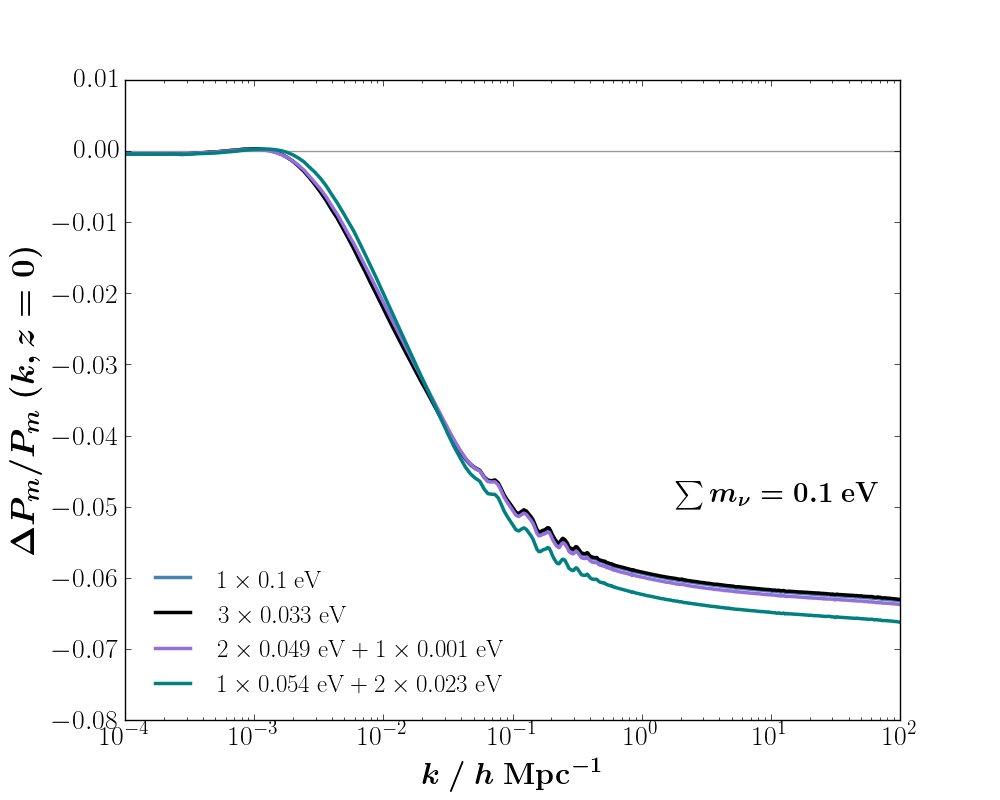
\includegraphics[width=0.8\columnwidth]{Ordering_Pk_linear.png}
\caption{Relative matter power spectrum at $z=0$ in the linear regime with respect to the neutrinoless CDM benchmark cosmology for 4 configurations of mass eigenstates of $\sum m_\nu = 0.1~\mathrm{eV}$: a single (`solo') eigenstate in blue, 3 degenerate eigenstates in black, 2 heavy + 1 light eigenstates (`inverted') in lavender, and 1 heavy + 2 light eigenstates (`normal') in green. }
\label{fig:pk_hierarchy}
\end{center}
\end{figure}

As the bounds on $\sum m_\nu$ close in on the $0.10~\mathrm{eV}$ upper limit where we can distinguish between normal and inverted orderings, it becomes increasingly critical to test the impact of mass hierarchy on the derived 1D flux power spectrum, which I'll introduce next chapter. In Sec.~\ref{sec:ordering_impact}, I present the resulting flux power spectra computed numerically with a suite of simulations described in Chap.~\ref{chap:Simulations} for three cases of $\sum m_\nu = 0.10~\mathrm{eV}$: normal and inverted orderings as well as the degenerate mass case. In the first two cases, the mass of each species is determined according to the squared mass differences of~\cite{Capozzi2013csa}. The individual masses in each case are given in Tab.~\ref{tab:ordering}. \\

\begin{table}
	\begin{center}
	\begin{small}
		\begin{tabular}{cccc}
			\textbf{configuration} & $\pmb{m_1 / \mathrm{meV}}$ & $\pmb{m_2 / \mathrm{meV}}$ & $\pmb{m_3 / \mathrm{meV}}$ \\[2pt]
			\hline \\[-10pt]
			solo & $100$ & $0$ & $0$ \\[2pt]
			inverted & $50$ & $49$ & $1$ \\[2pt]
			normal & $54$ & $24$ & $22$ \\[2pt]
			degenerate & $33$ & $33$ & $33$ \\[2pt]
			\hline \\[-10pt]
		\end{tabular}
	\end{small}
	\end{center}
	\caption{mass in meV of the three mass eigenstates $m_{1,2,3}$ from heaviest to lightest for a sum mass of $\sum m_\nu = 100 ~\mathrm{meV}$. The configuration labelled `solo' assumes a single non-zero mass eigenstate and two massless neutrinos. The `normal' and `inverted' ordering configurations have respectively 2 heavy + 1 light and 1 heavy + 2 light eigenstates, with mass differences in agreement with recent estimates from neutrino oscillations. The `degenerate' configuration assumes 3 indiscriminate eigenstates of $m_\nu^{\mathrm{eff}} = \sum m_\nu / 3$}
	\label{tab:ordering}
\end{table}

The linear matter transfer function is displayed in Fig.~\ref{fig:pk_hierarchy}. It can be noted that the differences in the linear 3D matter power spectrum are at the 0.1\% level between normal and degenerate orderings, and of order 0.3\% between inverted and degenerate configurations, quasi independently of $k$ scale  in the Ly-$\alpha$ forest range. The larger difference in the case of inverted ordering is explained by the fact that the total mass is essentially shared among two neutrinos instead of three for either the degenerate or the NH scenario. In the IH case, the lightest neutrino remains relativistic until late times: it becomes non-relativistic at around $z_{\mathrm{nr}} \sim 3$ for $\sum m_\nu=0.1$~eV. Thus, it contributes to the background density for longer spans of time, thereby leading to a slower growth of cold dark matter perturbations and to a stronger overall suppression of power. In contrast, the NH scenario having three neutrinos of almost equal masses is closer to the case of three degenerate-mass neutrinos. The slight bump and slope at $10^{-3} \lesssim k/h~\mathrm{Mpc}^{-1} \lesssim 10^{-1}$ relates an excess of power for the inverted compared to the normal or degenerate cases (and an excess of power of the normal ordering compared to degenerate), due to the presence of two (or one, respectively) higher-mass neutrinos, causing an earlier  non-relativistic transition and thus a free-streaming damping restricted to smaller scales. Relative to the degenerate case, the normal ordering (and even more so the inverted ordering) therefore exhibits an excess of power near $k_{\mathrm{nr}}\sim 10^{-3}~h~\mathrm{Mpc}^{-1}$. The tail of this peak is the cause of the slope near $k \simeq 10^{-2}~h~\mathrm{Mpc}^{-1}$ in Fig.~\ref{fig:pk_hierarchy}. The effects of individual masses are nevertheless small, of 0.3\% at most.


\begin{figure}
\begin{center}
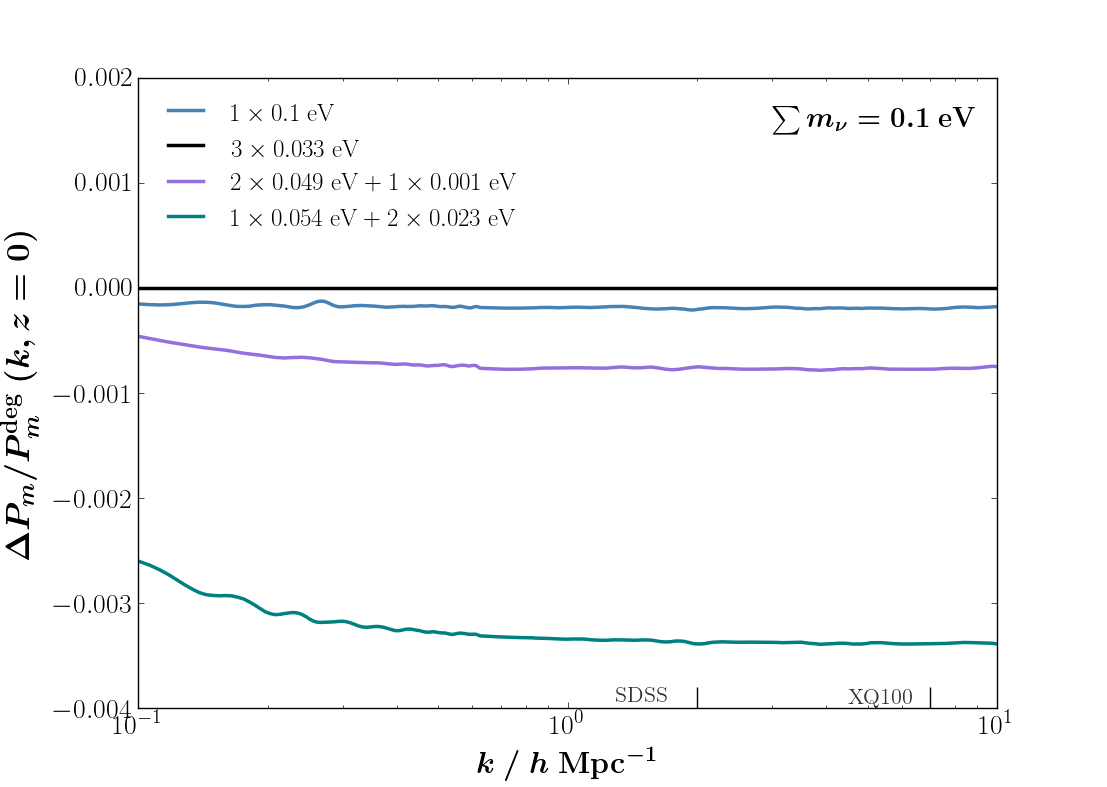
\includegraphics[width=0.8\columnwidth]{Ordering_Pk_zoom.png}
\caption{Zoom in on Fig.~\ref{fig:pk_hierarchy} on the range $0.1 \leqslant k/h~\mathrm{Mpc}^{-1} \leqslant 10$, with the reference model being the `degenerate' configuation (instead of the CDM benchmark model).}
\label{fig:pk_hierechy_zoom}
\end{center}
\end{figure}

\subsubsection{Cold+Warm Dark Matter}
\label{sec:cwdm_linear}

A wide class of NCDM dark matter models can be approximated by adding a CDM component in addition to, \textit{e.g.}, thermal WDM. Such models start to deviate from CDM at scales determined by the mass of WDM component, but the overall amount of suppression is controlled by the 
warm DM fraction, $F_{\rm{wdm}}$, of the total dark matter. The warm-to-total DM fraction can thus be defined such that \\
\begin{equation}
\Omega_{\rm{wdm}} = F_{\rm{wdm}} \times \Omega_{\rm{dm}} = F_{\rm{wdm}} \times \left( \Omega_{\rm{wdm}} + \Omega_{\rm{cdm}} \right) 
\label{eq:Fwdm}
\end{equation} \\ The solid and dashed transfer functions\footnote{$T(k) = \sqrt{P_{\rm{ncdm}}/P_{\rm{cdm}}}(k)$} at $z=0$ in Fig.~\ref{fig:pk_cwdm} feature the free-streaming cutoff scale for different NCDM masses. As discussed previously, heavier DM particles damp power on smaller scales, which makes them more consistent with the benchmark $\Lambda$CDM model, at least in the linear regime.
In a cold plus warm dark matter model (C+WDM), the smaller the fraction of the warm component, the colder the overall transfer function as is shown by the lighter colored lines in Fig.~\ref{fig:pk_cwdm} reaching an asymptotical plateau when $k \rightarrow \infty$ whose height is a function of the warm-to-cold fraction. For low $F_{\mathrm{wdm}} \lesssim 5~\%$ ratios, the plateau is well approximated by $1-T(k \rightarrow \infty) \sim (1-F_{\mathrm{wdm}})$ as demonstrated in \cite{BLR09}. \\

\begin{figure}
\begin{center}
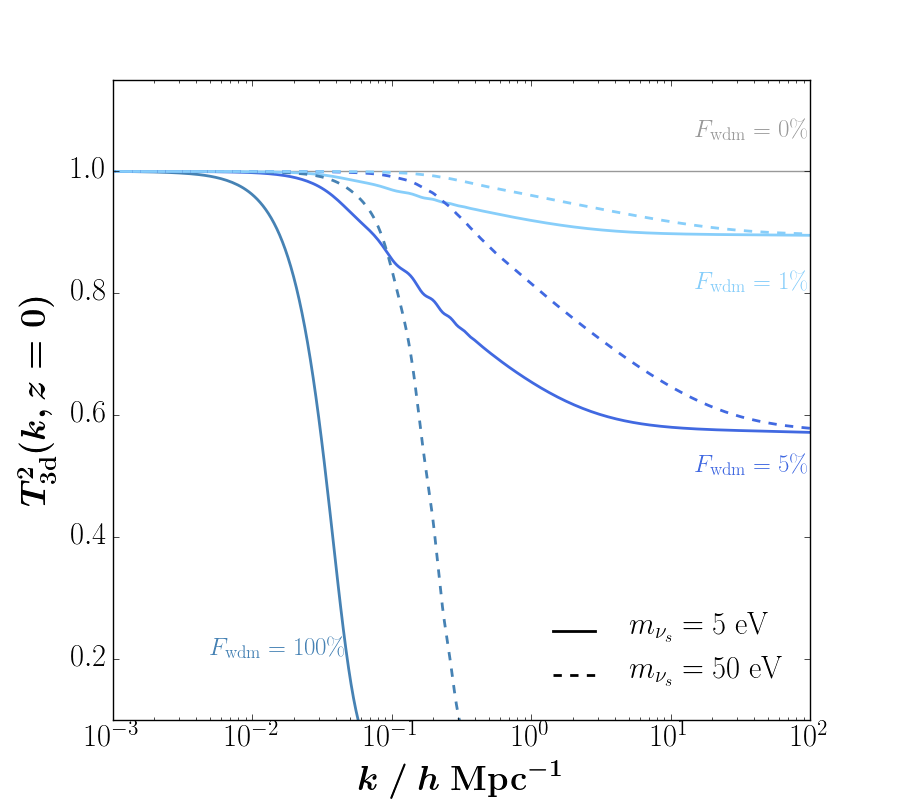
\includegraphics[width=0.8\columnwidth]{CWDM_T3D.png}
\caption{3D linear transfer function for total matter at $z=0$ computed by the \texttt{CLASS} software for $m_{\nu_s} = 5~\rm{eV}$ in solid lines and $m_{\nu_s} = 50~\rm{eV}$ in dashed lines. Dark teal lines assume a pure WDM model, and lighter tones of blue display a larger preponderance of the cold (heavier) component over the warm (lighter) one.}
\label{fig:pk_cwdm}
\end{center}
\end{figure}

The thermal velocities, \textit{i.e.} the velocity that defines the kinetic / internal energy, is given by the distribution function of the particle: \\
\begin{equation}
\int d^3q ~f(q) = \langle v \rangle ~\int d^3 q \frac{q}{\epsilon}~f(q)
\end{equation} \\ For masses of a few keV, the thermal velocities of WDM particles can be neglected (see Tab.~\ref{tab:vth}) and thus the total dark matter distribution can be treated as a mono-species collisionless fluid in our hydrodynamical simulations described in Chap.~\ref{chap:Simulations} whose linear transfer function is obtained by setting the DM abundance as $F_{\rm{wdm}}$ warm and $1-F_{\rm{wdm}}$ cold. The warm-to-total DM fraction $0 \leq F_{\rm{wdm}} \leq 1$ is therefore an additional free parameter that interpolates between the pure WDM limit ($F_{\rm{wdm}} = 1$) described above and the benchmark CDM ($F_{\rm{wdm}} = 0$) limit.


\begin{table}
	\begin{center}
	\begin{small}
		\begin{tabular}{cccc}
			$\pmb{m_x / \mathrm{keV}}$ & $\pmb{\langle v_{\mathrm{th}}^x \rangle (z=30)}$ & $\pmb{m_{\nu_s}^{\mathrm{nrp}} / \mathrm{keV}}$ & $\pmb{\langle v_{\mathrm{th}}^{\nu} \rangle (z=30)}$\\[2pt]
			\hline \\[-10pt]
			\\[-10pt]
			$1$ & $1.09~\mathrm{km}/s$ & $7$ & $0.70~\mathrm{km}/s$\\[2pt]
			$2.5$ & $0.32~\mathrm{km}/s$ & $10$ & $0.49~\mathrm{km}/s$\\[2pt]
			$5$ & $0.13~\mathrm{km}/s$ & $20$ & $0.24~\mathrm{km}/s$\\[2pt]
			$10$ & $0.05~\mathrm{km}/s$ & $30$ & $0.16~\mathrm{km}/s$\\[2pt]
			\hline \\[-10pt]
		\end{tabular}
	\end{small}
	\end{center}
	\caption{thermal velocities at $z=30$ for thermal relics and NRP sterile neutrinos as pure WDM}
	\label{tab:vth}
\end{table}


%%%%%%%%%%%%%%%%%%%%%%%%%%%%%%%%%%%%%%%%%%%%%%%%%%%%%
\subsection{Mapping Between Models}
%%%%%%%%%%%%%%%%%%%%%%%%%%%%%%%%%%%%%%%%%%%%%%%%%%%%%



\subsubsection{Mapping between Thermal Relics and Right-Handed Neutrinos}

In Sec.~\ref{sec:extrarad} and~\ref{sec:rhneu}, I explicited the distribution functions of the two main types of NCDM particles I consider throughout this work. Early decoupled thermal relics of mass $m_x$ and temperature $T_x$ on the one hand are Fermi distributed and contribute $\Delta N_\mathrm{eff} = (T_x/T_\nu)^4$ to the number of stable relativistic species coupled to photons early on in the Universe. NRP sterile neutrinos, on the other hand, display a quasi-Fermi distribution renormalized by $\vartheta \ll 1$ and contribute $\Delta N_{\mathrm{eff}} \propto \vartheta$. If one assumes that either one of those two make up the entirety of the dark matter, then given the similarities in their PSDs, one can establish a mapping between $m_x$ and $m_{\nu_s}$ since fixing $\Omega_x = \Omega_{\mathrm{dm}} = \Omega_{\nu_s}$ essentially normalizes the integral of the distribution functions over all momenta. Using Eqs.~\ref{eq:omnu} and~\ref{eq:omx}, one can relate \\
\begin{equation}
m^{\mathrm{eff}}_\nu = \begin{cases}
%\Sigma m_\nu & \text{for lepton neutrinos}\\
\vartheta ~\times~ m_{\nu_s} & \text{for sterile neutrinos}\\
\left( \cfrac{T_x}{T_\nu} \right)^3 \times m_x & \text{for thermal relics}
\end{cases}
\end{equation} \\ or, equivalently,\\
\begin{equation}
\label{eq:neff_whether}
N_{\mathrm{eff}} = \begin{cases}
\cfrac{m_\nu^\mathrm{eff}}{m_{\nu_s}} & \text{for sterile neutrinos}\\
\left( \cfrac{m_\nu^\mathrm{eff}}{m_x} \right) ^{4/3} = \left( \cfrac{T_x}{T_\nu} \right)^4 & \text{for thermal relics}
\end{cases}
\end{equation} \\ Using the \texttt{CAMB} software to produce the transfer functions of a thermal relic of mass $m_x$ is encoded in the $\Delta N_\mathrm{eff}$ it contributes. The same $\Delta N_\mathrm{eff}$ is obtained assuming the dark matter is a NRP neutrino of mass $m_{\nu_s}$ such that \\
\begin{empheq}[box=\mymath]{equation}
m_{\nu_s} = \kappa ~ m_x^{\mu} / \omega_{\rm{wdm}}^{1/3}
\label{eq:mxms}
\end{empheq} \\ where $\omega_{\rm{wdm}} = F_{\rm{wdm}} \times \Omega_{\rm{dm}}h^2$ is expressed in units of $0.25 \times 0.7^2$. The authors of \cite{VLH08a} issue $\kappa = 4.43~\rm{keV}$ and $\mu = 4/3$; whereas the authors of \cite{Abazajian2016} issue a mapping with $\kappa = 3.90~\rm{keV}$ and $\mu = 1.294$ by accounting for the non-uniform value of $g_\star$ throughout the production mechanism of sterile neutrinos as well as the thermodynamics of the QCD phase transition. Eq.~\ref{eq:mxms} will be used hereafter whenever deriving limits on the mass of thermal relics and sterile neutrinos. \\


\begin{figure}
\begin{center}
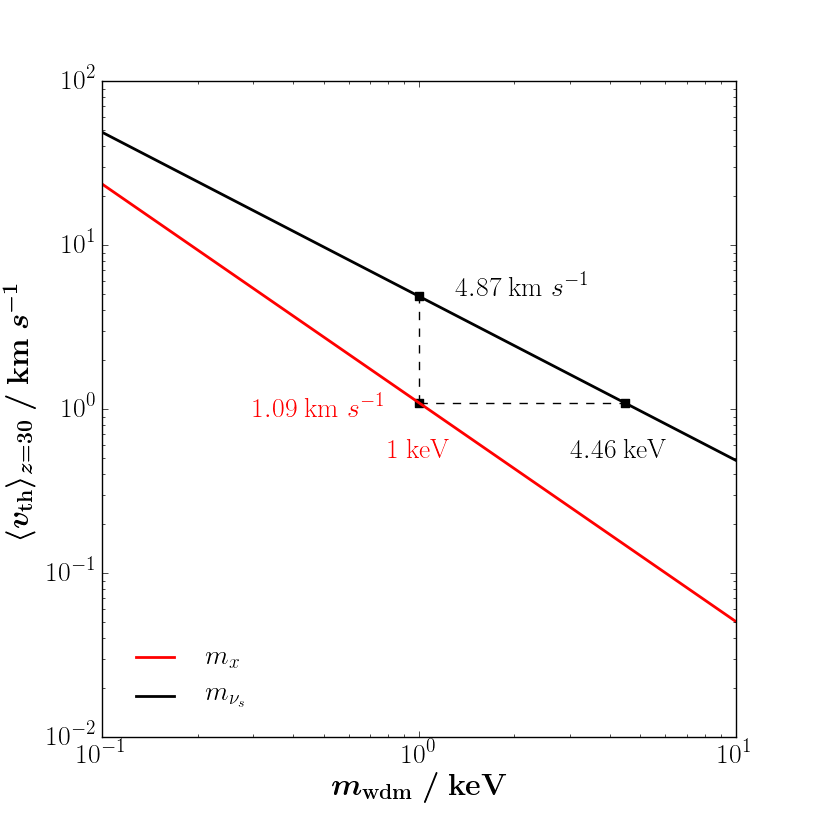
\includegraphics[width=0.8\columnwidth]{thermal_velocity.png}
\caption{thermal velocities of WDM particles at $z=30$, for an early decoupled thermal relic (red) and a non-resonantly produced sterile neutrino (black).}
\label{fig:thermal_velocity}
\end{center}
\end{figure}

In Fig.~\ref{fig:thermal_velocity}, I display the value of the thermal velocity of the WDM candidate particle as a function of its mass. The mapping can be interpreted as is illustrated on this figure. Both a $m_x=1~\mathrm{keV}$ thermal relic and a $m_{\nu_s} = 4.46~ \mathrm{keV}$ NRP neutrino have a thermal velocity at $z=30$ of $1.09~ \mathrm{km}/s$, and so their free-streaming horizon scales are identical, as are their transfer functions. A $m_{\nu_s} = 1~\mathrm{keV}$ NRP sterile neutrino on the other hand, has a thermal velocity of $\langle v \rangle (z=30) = 4.87~\mathrm{km}/s$. \\

I would like to attract the reader's caution when using Eq.~\ref{eq:mxms} as it only pertains to the warm component of the dark matter, not the total population. Hence, when producing C+WDM models, the mass mapping between $m_x$ and $m_{\nu_s}$ is a function of $F_{\mathrm{wdm}}$. Fig~\ref{fig:mx_ms_withF} displays the value of a NRP sterile neutrino that contributes the same $\Delta N_\mathrm{eff}$ as a thermal relic of mass $m_x$ for a given fraction $F_{\mathrm{wdm}}$. Notice that, for instance, in the second to last column, a $m_x = 1~ \mathrm{keV}$ relic maps to a $m_{\nu_s} \simeq 3.9~\mathrm{keV}$ NRP neutrino in the pure WDM case (as is conformal to  Eq.~\ref{eq:mxms} with the mapping of \cite{Abazajian2016}). However, that same $m_x = 1~ \mathrm{keV}$ relic maps to a $m_{\nu_s} \simeq 10.7~\mathrm{keV}$ NRP neutrino in a C+WDM model with $\Omega_{\mathrm{wdm}} = 5\% \times \Omega_{\mathrm{dm}}$.  \\

\begin{figure}
\begin{center}
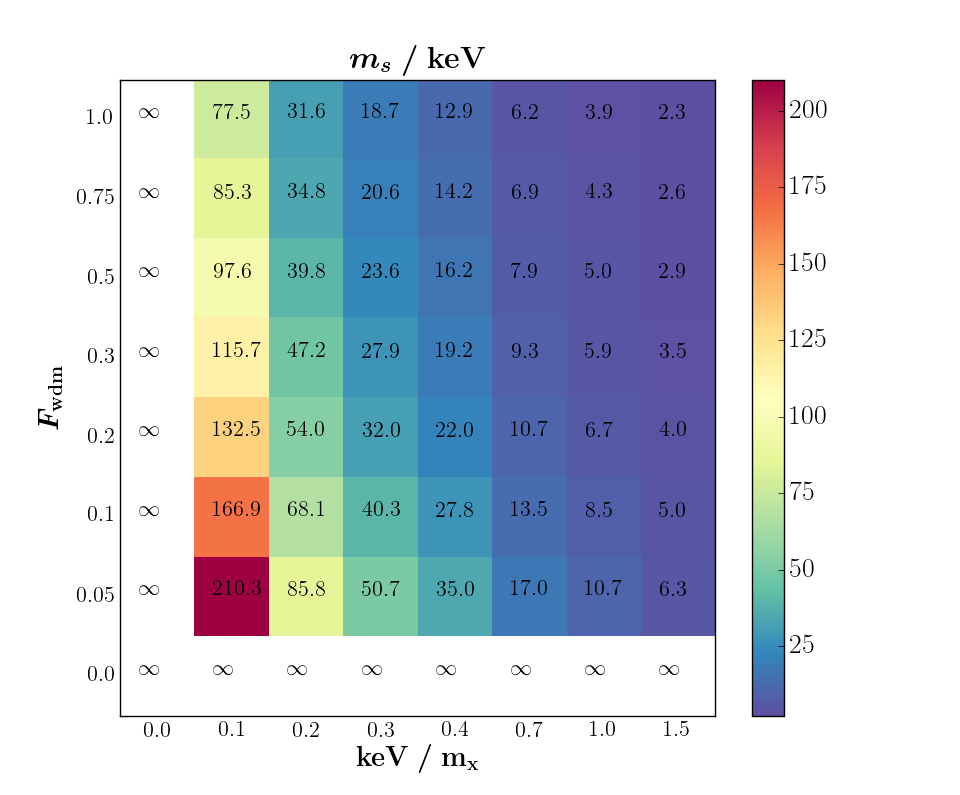
\includegraphics[width=0.9\columnwidth]{Map/MX_to_MS.png}
\caption{Value of $m_{\nu_s}$ as a function of $\left( \mathrm{keV}/m_x, F_\mathrm{wdm} \right)$ in the context of a C+WDM cosmology.}
\label{fig:mx_ms_withF}
\end{center}
\end{figure}

Of course, since RPSN have strongly non-thermal distribution functions, this mapping is invalid when one tries to relate $m_x$ and $m_{\nu_s}^{\mathrm{rp}}$ when $\mathcal{L} > 0$.

\subsubsection{Mapping between Cool and Warm+Cold}
\label{sec:map_rpsn_cwdm}

Both C+WDM and RPSN as cool DM feature similar transfer functions up to a certain $k$ scale. One can thus use both cosmologies to produce a mapping of sorts in between $\left( m_{\nu_s}^{\mathrm{nrp}}, F_{\mathrm{wdm}} \right)$ and $\left( m_{\nu_s}^{\mathrm{rp}}, \mathcal{L} \right)$ assuming $F = 1$ for the latter and $\mathcal{L}=0$ for the former. \\ 

\begin{figure}
\begin{center}
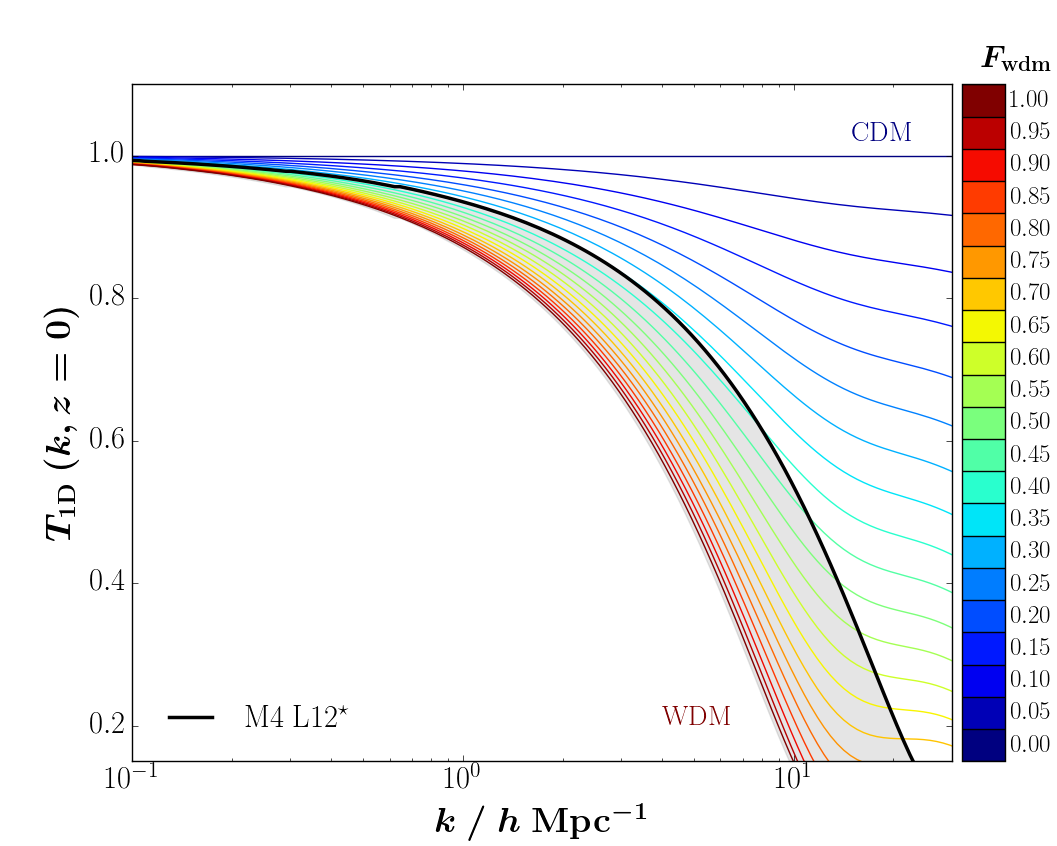
\includegraphics[width=0.75\columnwidth]{RPSN/T1D_M04.png}
\caption{ 1D linear transfer function for the total matter at $z=0$ obtained with the \texttt{CLASS} software for a DM made of a $4~\rm{keV}$ sterile neutrino. The color encodes the warm-to-total fraction $0 \leq F_{\rm{wdm}} \leq 1$, which ranges from the warmest (pure WDM) to the coolest (CDM) cases. Considering sterile neutrino pure cool dark matter, the transfer functions for the $0 \leq \mathcal{L} \leq \mathcal{L}^\star$ and $\mathcal{L}^\star \leq \mathcal{L} \leq \mathcal{L}^{\mathrm{max}}$ RPSN are all contained within the shaded grey region, bounded by the warmest and coolest models, respectively $\mathcal{L}=0$ (NRP in dark red) and $\mathcal{L}^\star = 1.2 \times 10^{-5}$ for $m_{\nu_s} = 4~\rm{keV}$ in thick black. }
\label{fig:M4t1d}
\end{center}
\end{figure}

Fig.~\ref{fig:M4t1d} illustrates the correspondance between the coolest RPSN model of 4 keV ($\mathcal{L}^\star = 1.2 \times 10^{-5}$) and the 4 keV neutrino produced in absence of a lepton asymmetry that constitutes $\sim 35\%$ of the total dark matter. The correspondance is obtained with a least-square method out to $k_{\rm max} = 1.35\,h^{-1}{\rm Mpc}$ on the linear transfer function. Because Ly-$\alpha$ forests are a unidimensional probe for the matter distribution, I perform the mapping on the 1D transfer function, obtained using Eq.~\ref{eq:1dpwrspctrm}, and with $T^2_{\mathrm{1d}} (k) = P_{\mathrm{1d}}^{\mathrm{ncdm}} / P_{\mathrm{1d}}^{\mathrm{cdm}}$. This $\mathcal{L}-F_{\mathrm{wdm}}$ mapping enables me to convert the bounds on ($m_{\nu_s}$, $F_{\rm{wdm}}$) to bounds on ($m_{\nu_s}$, $\mathcal{L}$). Fig.~\ref{fig:L_to_F_map} displays the value of $F_{\mathrm{wdm}}$ that yields the most similar 1D transfer function for a given mass for all of the $16 \times 30$ RPSN models we have at our disposal, using the \texttt{CLASS} software with the PSDs from \cite{LaineMSM, Ghiglieri2015jua}. Notice the region corresponding to the lowest mixture of warm-to-cold fraction (in blue) has the same shape than the region in Fig.~\ref{fig:rpsn_banana} which displays the lowest values of $\langle q \rangle / m$ for a given mass. This is hardly a coincidence, since both relate to the free-streaming horizon scale. \\

\begin{figure}
\begin{center}
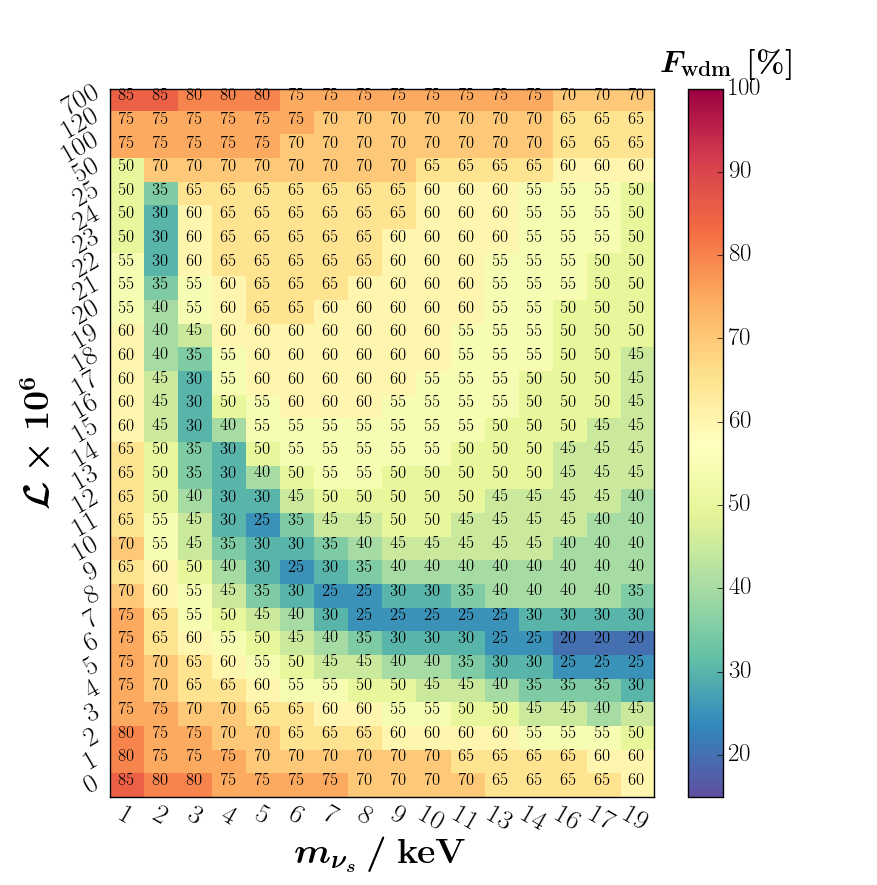
\includegraphics[width=0.8\columnwidth]{Map/L_to_F_BOSS.png}
\caption{Mapping between $\left( m_{\nu_s}^{\mathrm{nrp}}, F_{\mathrm{wdm}} \right)$ assuming $\mathcal{L}=0$ (C+WDM) and $\left( m_{\nu_s}^{\mathrm{rp}}, \mathcal{L} \right)$ assuming $F_{\mathrm{wdm}}=1$ (pure cool dark matter). The numerical values and color code correspond to the value of $F_{\mathrm{wdm}}$ whose C+WDM 1D transfer function issues the least square with the RPSN 1D transfer function of the same DM particle mass, as illustrated in Fig.~\ref{fig:M4t1d}}
\label{fig:L_to_F_map}
\end{center}
\end{figure}

It is noteworthy to mention that this mapping is done in the linear regime only. In Sec.~\ref{sec:mapping_flux_RPSN_CWDM}, I verify that this mapping holds for the non-linear regime, when computing the power spectrum with the Ly-$\alpha$ forest, at least on scales probed by our set of data. 

